\documentclass[preprint,12pt]{elsarticle}

% Latin Modern before anything else: elsarticle's default T1-encoded Computer
% Modern has no Type 1 outlines on many installations, so pdfTeX silently
% substitutes Type 3 bitmaps -- which publisher PDF-compliance checks reject.
% lmodern supplies Type 1 outlines for the same design. Do not remove.
\usepackage{lmodern}
\usepackage[T1]{fontenc}

\usepackage{amsmath,amssymb,amsfonts}
\usepackage{amsthm}          % elsarticle provides no proof environment
\usepackage{graphicx}
\usepackage{tikz}
\usetikzlibrary{arrows.meta,positioning,calc}
\usepackage{lineno}
\usepackage{array}         % >{\raggedright} column prefixes, so a
                           % narrow table column breaks instead of
                           % overfilling
\newcolumntype{R}[1]{>{\raggedright\arraybackslash}p{#1\textwidth}}
\usepackage{url}           % elsarticle loads neither url nor
                           % hyperref; \url breaks the repository
                           % address, \texttt would overfull it

% The submission layout is single-column, but the journal sets two columns, and
% a narrow measure full of long technical words overflows. Let TeX stretch the
% inter-word space instead; harmless in the wide layout, and it clears the
% overfull boxes in the narrow one.
\tolerance=1500
\emergencystretch=2em
\hyphenpenalty=100
\hbadness=4000

\theoremstyle{plain}
\newtheorem{theorem}{Theorem}[section]
\newtheorem{lemma}[theorem]{Lemma}
\newtheorem{proposition}[theorem]{Proposition}
\newtheorem{corollary}[theorem]{Corollary}
\newtheorem{remark}[theorem]{Remark}

\newcommand{\R}{\mathbb{R}}
\newcommand{\E}{\mathbb{E}}
\newcommand{\dvec}{\mathbf{d}}
\newcommand{\dhat}{\hat{\mathbf{d}}}
\newcommand{\Var}{\mathrm{Var}}
\newcommand{\Std}{\mathrm{Std}}
\newcommand{\dFR}{d_{\mathrm{FR}}}
\newcommand{\DB}{D_{\mathrm{B}}}
\newcommand{\lloss}{\ell}

\journal{Reliability Engineering \& System Safety}

\begin{document}

\begin{frontmatter}

\title{Information loss of fixed linear health indicators as a control problem:
simplex geometry and reachability limits}

\author[a]{Huy Hoang Le}
\ead{lhhoang@powermore.vn}
\author[b]{Kim-Anh Nguyen\corref{cor}}
\ead{nkanh@dut.udn.vn}
\cortext[cor]{Corresponding author}
\affiliation[a]{organization={R\&D Department, PowerMore Ltd.},
  city={Da Nang}, postcode={550000}, country={Viet Nam}}
\affiliation[b]{organization={Faculty of Electrical Engineering, University
  of Science and Technology, The University of Danang},
  city={Da Nang}, postcode={550000}, country={Viet Nam}}

\begin{abstract}
A health indicator compresses several condition-monitoring channels into one
scalar, and normally keeps the same weights for the life of the component.
We take it to be a fixed linear map of noise-whitened channels on which every mechanism acts positively, over a population whose units differ only in where they sit on one degradation path, with remaining life Gaussian across it.
Because degradation runs through several mechanisms at differing rates, the
channel combination carrying most information about remaining life rotates as
the component ages, so a fixed indicator necessarily discards information. We
show that the operating point sets how much it discards, which makes that loss
a control variable. The loss reduces to a single angle, between the indicator and the direction along which information currently arrives, and writing each channel's share of that information as a probability vector places that angle on a statistical simplex. Zero loss is attainable exactly when the
directions reachable at each instant share a common point, which for generic
plants needs one fewer independently adjustable operating variable than there
are mechanisms. Scaling every channel by the same factor leaves the loss
unchanged, so no criterion built from the Fisher information about
remaining life can detect it. Steering the operating point reduces the loss substantially when the authority it offers is large beside the drift of the informative direction; on a representative three-mechanism synthetic plant the information-loss objective defined here falls by a factor of $68$ against the best constant operating point. A dimensionless index of that balance, available before any indicator is chosen, describes the regime rather than deciding it, with an area under the receiver-operating curve of $0.73$ over $299$ random plants. Six public run-to-failure fleets test the premises separately: an informative direction estimated from measured cells rotates, and simulated turbofan records confirm against a negative control that the operating point moves it. The same fleets bound the theory: the highest-fidelity turbofan data reject the separable plant form under which the operator's authority becomes computable offline, so that branch describes a model class rather than measured machinery.
\end{abstract}

\begin{keyword}
prognostics \sep health indicator \sep remaining useful life \sep
information loss \sep optimal control \sep reachability
\end{keyword}

\end{frontmatter}

\linenumbers

\section{Introduction}
\label{sec:intro}

Condition monitoring rarely feeds raw measurements to a life-prediction
algorithm. A vibration channel, a temperature, an impedance and a capacity
reading first go into a single scalar, the health indicator, and the
life-prediction algorithm sees only that scalar~\cite{lei2018,coble2009}. The
compression is almost always fixed: the designer picks one set of weights at
design time, and every unit carries those weights for its whole life, because
firmware embeds them, certification freezes them, or re-tuning them in the
field is impractical.

Fixing the compression has a cost. Real components degrade through several
mechanisms at once, and those mechanisms do not proceed in step: an early-life
process may dominate for the first third of the record and then saturate,
while a late-life process accelerates. The combination of channels that
carries the most information about remaining life therefore rotates as the
component ages. A fixed indicator is aligned with that combination at best at
one moment, and is misaligned for the rest of the record; the information it
discards is not recoverable downstream, however good the prediction algorithm
that follows~\cite{le2026jestech}.

The established response is to make the map better: choose a different
criterion for it, let it switch between segments of life, or learn it from
more run-to-failure data~\cite{le2026mst,coble2009}. All of these take the degradation as given and work on the compression. This paper acts on the degradation itself, through the operating point.

The rotation is not a property of the instrumentation. The degradation physics
produces it, and that physics responds to stress: temperature, load and duty
cycle change the relative rates of the competing mechanisms, not only the
overall speed. Running a cell hotter does not only age it faster; it also
shifts the balance between the mechanisms, and therefore moves the direction
in which information about remaining life arrives.

The operating point is, in most applications, something the operator chooses.
So the misalignment between a fixed indicator and the informative direction is
not fixed by nature. It is a function of the input, and the operator can steer
it.

That reframing turns a data-analysis question into a control question, and
control questions come with sharper answers than design heuristics do. One can
ask what misalignments are reachable at a given operating envelope, whether
zero loss is attainable at all, how many independent inputs that would take,
and what the best achievable loss is when it is not. These are the questions
this paper answers.

They sit against five bodies of work. Four address parts of the problem and
the fifth supplies the geometry used in Section~\ref{sec:simplex}; to our knowledge none of them addresses the position taken here.

The prognostics literature treats the compression as a design problem to be
solved from data: searching genetically over candidate features against
monotonicity and trendability criteria~\cite{coble2009}, learning it with a
recurrent network~\cite{guo2017}, or surveying the resulting
pipelines~\cite{lei2018,javed2017}. Two limits on that programme are known, information-theoretic bounds on what any fixed compression can retain~\cite{le2026jestech} and the number of run-to-failure units needed to learn one reliably~\cite{le2026mst}. The first is our own, and the boundary is worth drawing explicitly: it takes one degradation trajectory as given and asks how much information a fixed compression must lose along it. The question here is the complementary one, whether that trajectory can itself be steered so that the same fixed map loses less. Both prior limits hold the trajectory fixed; neither asks whether it can be changed.

The predictors downstream are overwhelmingly stochastic --- Wiener, gamma and
inverse-Gaussian degradation processes with first-passage
failure~\cite{ye2015,noortwijk2009}, reviewed for remaining-life estimation
in~\cite{si2011,zhang2018} and embedded in system-level design methodology
in~\cite{lee2014}. That literature models how damage evolves, not how the
measurement should be compressed before the model is applied, which is the
question upstream of it.

A separate literature does treat the operating point as a decision variable,
but to extend remaining life rather than to preserve
estimability~\cite{hac2020,rulcontrol2025}; the two aims can conflict, and
Section~\ref{sec:num} exhibits an instance in which they disagree. Choosing
inputs to make a state easier to estimate is itself classical, going back to
dual control~\cite{feldbaum1960}, and its modern forms shape a scalarisation
of the Fisher information matrix~\cite{oato2021,hooker2015,adt2011}. Our
Proposition~\ref{prop:blind} shows the quantity at issue here to be invisible
to every such scalarisation.

The fifth body is information geometry. The reformulation of
Section~\ref{sec:simplex} rests on the Fisher--Rao geometry of the probability
simplex and on the Bhattacharyya
coefficient~\cite{amari2016,bhattacharyya1943}, and the flow it produces is
the replicator equation of evolutionary
dynamics~\cite{hofbauer1998,sandholm2010}. These are standard objects; what is
new here is their identification with the informative direction of a degrading
component, and the fact that the fitness driving the flow is actuated.

\begin{table*}[t]
\caption{Where this paper sits. The columns are the axes that separate these
literatures, not a ranking: each body of work answers a question the others do
not ask, and the last column is a restriction this paper imposes on itself
rather than an advantage over the others. ``Input alters degradation'' means
the operating point enters the degradation dynamics; ``direction'' means the
informative direction of Section~\ref{sec:prelim} is itself an objective.}
\label{tab:position}
\centering
\footnotesize
\setlength{\tabcolsep}{3pt}
\begin{tabular}{@{}R{0.34}cccc@{}}
\hline
 & input alters & lifetime is & direction is & indicator\\
 & degradation & an objective & an objective & fixed, scalar\\
\hline
Indicator design~\cite{coble2009,guo2017,lei2018} &
  --- & --- & --- & $\checkmark$\\
Fixed-indicator limits~\cite{le2026jestech,le2026mst} &
  --- & --- & --- & $\checkmark$\\
Stochastic life models~\cite{ye2015,si2011} &
  --- & --- & --- & ---\\
Health-aware control~\cite{hac2020,rulcontrol2025} &
  $\checkmark$ & $\checkmark$ & --- & ---\\
Observability-aware~\cite{feldbaum1960,oato2021,adt2011} &
  $\checkmark$ & --- & partly & ---\\
\hline
This paper & $\checkmark$ & secondary & $\checkmark$ & $\checkmark$\\
\hline
\end{tabular}
\end{table*}

The contributions are as follows.

\begin{enumerate}
\item The information a fixed indicator discards is an exact function of one
misalignment angle (Lemma~\ref{lem:exact}). Placing the channels' shares of
the Fisher information on a statistical simplex turns the degradation into a
replicator flow whose rates the operating point modulates, and the optimal
indicator into a barycentre of the degradation path
(Section~\ref{sec:simplex}).

\item Zero loss is attainable exactly when the reachable direction sets share a
point, which generically needs at least as many independent operating
variables as mechanisms less one (Section~\ref{sec:reach}). Supplying the
missing input collapses the peak reachability floor from $4.52^{\circ}$ to
zero at every state, so the rule prices instrumentation rather than only
bounding it. Taking logarithms makes every reachable set a translate of one
fixed set, which turns the question into a containment and shows the counting
rule to be sufficient but not necessary; the exceptions exist for any number of mechanisms and are too fragile to build on (Section~\ref{sec:translate}). The count separates two objectives that are easily conflated: holding the misalignment at a constant level is a single scalar condition and generically needs one input, whereas freezing the informative direction outright is $d-1$ conditions. That gap is the difference between useful steering and lossless steering, and an installation with one controllable variable can have the first without the second.

\item The loss is invariant to a common gain on all channels and is therefore
invisible to every scalarisation of the Fisher information about remaining
life, so no criterion built from that information alone can rank indicators by
the loss they incur.

\item The best achievable loss is the value of an optimal control problem
whose objective is a ratio, and whose terminal time is itself controlled
(Section~\ref{sec:limit}); we compute its value to two digits and do not certify it. A dimensionless regime index, computable before any indicator is designed, describes the regime in which steering can have substantial value, and its accuracy and the direction of its errors are measured on $299$ randomly drawn plants (Section~\ref{sec:regime}).

\item The premises are separately testable on public run-to-failure
data, and Section~\ref{sec:scope} tests three in turn: whether the informative
direction rotates, whether the operating point moves it, and whether the
separable stress model survives. The first holds on measured fleets, the
second so far only in simulation, and the third is rejected. That section
therefore reports which hypotheses withstand contact with data rather than
demonstrating that the method works.
\end{enumerate}

The results do not all rest on the same assumptions, and it is worth
separating them before any of them is stated. Lemma~\ref{lem:exact},
Proposition~\ref{prop:record} and Theorem~\ref{thm:zero} need only the
observation model of Section~\ref{sec:prelim}: a fixed linear indicator on
whitened channels, and a scalar latent. Lemma~\ref{lem:sep} and
Proposition~\ref{prop:contain} need more, namely that the input enters each
mechanism through a single separable factor, and Section~\ref{sec:scope}
reports that the highest-fidelity turbofan data reject exactly that. The
empirical readings of Section~\ref{sec:scope} need more again, since
estimating one informative direction from a fleet presumes the units differ by
a time shift rather than by their degradation coefficients.
Fig.~\ref{fig:scope} is the map, and the reader who wants to know which branch
a given result sits on should consult it rather than infer it.

Section~\ref{sec:prelim} states the model. Sections~\ref{sec:simplex}
to~\ref{sec:limit} develop the theory, Section~\ref{sec:num} exercises the
three of its claims that are stated sharply enough to be refuted, and
Section~\ref{sec:scope} reports what public fleet data can and cannot
establish about the premises the theory rests on.

\section{Problem formulation}
\label{sec:prelim}

This section states the degradation model, says precisely what a prognostic
algorithm is being asked to estimate and where the uncertainty in that
quantity comes from, derives the direction along which information about it
arrives, and defines the fixed indicator whose information loss the rest of
the paper studies. Readers familiar with~\cite{le2026jestech} will recognise
the model; the derivation is given in full here because the geometry of
Section~\ref{sec:simplex} depends on several of its details.

\subsection{Degradation driven by a controlled operating point}

A component degrades through $d$ distinct mechanisms acting at once. In a
lithium-ion cell these might be loss of cyclable lithium, growth of the
solid-electrolyte interphase and mechanical fatigue of the electrode; in a
rolling bearing, spalling, wear and lubricant degradation. We write $x_i(t)
\ge 0$ for the damage accumulated by mechanism $i$ up to time $t$, and collect
these into the state $x=(x_1,\dots,x_d)$.

One externally chosen operating point drives all $d$ mechanisms. It collects
the temperature, the mechanical or electrical load, and the duty cycle at
which the operator runs the component. We write that operating point as
\begin{equation}
u(t)\in\mathcal U\subset\R^{m},
\label{eq:input}
\end{equation}
with $\mathcal U$ compact, representing the operating envelope the application
permits. Throughout this paper $u$ is the control input: it is the decision
variable, and the question we ask is what choosing it well can buy. The number
of independent inputs, $m$, turns out to decide what is achievable, and it is
usually much smaller than the number of mechanisms $d$.

The damage states evolve according to
\begin{equation}
\dot x_i=\varphi_i(u)\,h_i(x_i),\qquad i=1,\dots,d,
\label{eq:plant}
\end{equation}
in which the two factors play different roles:
\begin{itemize}
\item $\varphi_i(u)>0$ is the stress-acceleration factor of mechanism
$i$: how much faster that mechanism runs at operating point $u$ than at a
reference point. It carries all the dependence on the input.
\item $h_i(x_i)>0$ is the intrinsic shape of mechanism $i$: how its
rate depends on the damage it has already done. It carries all the dependence
on the state.
\end{itemize}
This separation is the standard accelerated-life form and covers the stress
models in routine use~\cite{meeker1998}. In the Arrhenius model the input is
absolute temperature and $\varphi_i(u)=A_i\exp\!\big(-E_i/(k u)\big)$, with
$A_i>0$ a pre-exponential constant, $E_i>0$ the activation energy of mechanism
$i$ and $k$ Boltzmann's constant. In the inverse-power-law model the input is
a mechanical or electrical stress and $\varphi_i(u)=\kappa_i u^{\,n_i}$, with
$\kappa_i>0$ a scale factor and $n_i>0$ the stress exponent. Choosing $h_i$
recovers the exponential, power-law and stretched-exponential degradation
classes~\cite{le2026jestech}; the results below use only $\varphi_i>0$ and
$h_i>0$.

The within-unit dynamics are deterministic, where most of the degradation
literature places the randomness inside a single unit's
path~\cite{ye2015,noortwijk2009,zhang2018}. We put it between units instead
(Section~\ref{sec:R}). The object of study is the direction along which
information arrives, which is fixed by the relative rates of the competing
mechanisms: a within-unit diffusion would jitter that direction without
altering its systematic motion, whereas dispersion in the rate parameters
across a population is what makes remaining life uncertain and therefore worth
estimating.

We measure damage on a scale normalised so that mechanism $i$ exhausts the component's tolerance when $x_i$ reaches unity. A component is withdrawn at a condemnation limit at or below that point, so we write the end of life as the first passage of any one mechanism to a threshold $x_f\in(0,1]$:
\begin{equation}
T_f=\inf\{t\ge0:\textstyle\max_i x_i(t)\ge x_f\}.
\label{eq:tf}
\end{equation}
No result below depends on the value of $x_f$, which enters only by fixing where a trajectory stops. The computed quantities of Section~\ref{sec:num} do depend on it, and the value used there is stated with the rest of the test plant.

\subsection{What is to be estimated, and why it is uncertain}
\label{sec:R}

The quantity a prognostic system must report is the remaining useful life
\begin{equation}
R(t):=T_f-t,
\label{eq:R}
\end{equation}
the time left before failure.

We must say where the uncertainty in $R$ lies, because \eqref{eq:plant} is a
deterministic differential equation: for one component whose initial damage
and parameters were known exactly, $T_f$ and hence $R$ would be known exactly,
and there would be nothing to estimate. The uncertainty is between components,
not within one. Units built to the same specification differ in initial damage
and in the coefficients of \eqref{eq:plant}, which is the unit-to-unit
variability that reliability engineering treats as the primary source of
scatter in life data~\cite{meeker1998}. A prognostic algorithm observes one
unit drawn from that population and must infer its remaining life.

We therefore treat $R$, at any given observation instant, as a random variable
over the population of units, with prior variance $\Var[R]>0$. This variance
is the uncertainty the algorithm exists to reduce, and it is the reason the
estimation problem is not trivial. Everything below is written for a nominal
trajectory of \eqref{eq:plant}, with the fleet spread entering only through
$\Var[R]$.

\subsection{Observations and the informative direction}
\label{sec:dvec}

Each damage state reaches the record through its own noisy channel,
\begin{equation}
y_i=x_i+\sigma_i\epsilon_i,\qquad i=1,\dots,d,
\label{eq:obs}
\end{equation}
with $\sigma_i>0$ the noise level of channel $i$ and $\epsilon_i$ independent standard normal variables. The record available to the algorithm is the collection of these measurements over the observation window.

Equation~\eqref{eq:obs} pairs each mechanism with a channel of its own. Condition monitoring in general returns $y=H(x,u)+\epsilon$, with sensors that mix mechanisms, and the pairing is an assumption rather than a description. It is load-bearing: the positivity of $\dvec$ that Remark~\ref{rem:pos} shows the results to need follows from $\varphi_i>0$ and $h_i>0$ in these coordinates and need not survive an arbitrary $H$. Where $H$ is known, invertible and positivity-preserving the construction carries over to $H^{-1}y$; the general case does not reduce to it.

Two assumptions carry the sensitivity, and both are stated here rather than left to be inferred.

\paragraph{The prior on $R$} We take $R$ to be Gaussian over the population with variance $\Var[R]$. Linearising the record about the nominal trajectory, following~\cite{le2026jestech}, then makes the record and $R$ jointly Gaussian, and the mutual informations below are exact. Linearisation alone would not do it: with a non-Gaussian prior of the same variance the Gaussian value is an upper bound on what a channel carries, and Lemma~\ref{lem:exact} becomes an inequality rather than an identity. The information geometry that follows is exact under this Gaussian prior and the time-shift population described next; it is not a model of population variability in general.

\paragraph{How units differ} We take the population spread to be a reparametrisation of a single degradation path: units differ in where they sit on the trajectory of \eqref{eq:plant}, not in its shape. This is what makes $R$ a coordinate along that path, and it is what the next display uses. Dispersion in the coefficients of \eqref{eq:plant} is a different matter, because it moves $\partial x/\partial\theta$ rather than sliding along $\partial x/\partial R$, and Remark~\ref{rem:shift} records what it costs.

The sensitivity of channel $i$ to remaining life then follows from \eqref{eq:R}: because $R$ falls at unit rate as $t$ advances,
\begin{equation}
\frac{\partial x_i}{\partial R} =-\frac{\partial x_i}{\partial t}
=-\varphi_i(u)\,h_i(x_i).
\label{eq:sens}
\end{equation}
\begin{remark}[what the time-shift assumption costs]\label{rem:shift}
Equation~\eqref{eq:sens} is exact when the population spread slides along one path, and only then. On the plant of Section~\ref{sec:testplant}, with units instead drawn by dispersing the degradation coefficients, the direction that the population regression of $x$ on $R$ actually returns stands about $45^{\circ}$ from $-\varphi(u)h(x)$, across two families of dispersed coefficient and every spread tried; a control whose units are started on the reference trajectory, where \eqref{eq:sens} holds by construction, returns the same regression to within $0.2^{\circ}$. The misalignments this paper is about are a few degrees. Extending the construction to populations dispersed in $\theta$, where the observation carries scatter that no value of $R$ explains, is open.
\end{remark}

Dividing each channel by its own noise level puts them on a common scale, and
taking magnitudes gives the whitened signal direction
\begin{equation}
\dvec(t)=\big[\sigma_i^{-1}\varphi_i(u)h_i(x_i)\big]_{i=1}^{d}, \qquad
\dhat=\dvec/\|\dvec\| .
\label{eq:dvec}
\end{equation}
In words: $\dvec$ says how strongly, and in what combination of channels, the
measurement responds to a change in remaining life. Its direction $\dhat$ is
the \emph{informative direction}, the combination a health indicator has to be
aligned with and the object named informally in Section~\ref{sec:intro}. Its length $\|\dvec\|$ is the strength of that signal. The two objects carry the paper: $\|\dvec\|$ is how much information arrives and $\dhat$ is where it arrives from, and the loss of a fixed indicator depends only on the second. Experiment design in the observability tradition scores the first, which is why Proposition~\ref{prop:blind} finds it blind to the loss.

We use two properties of \eqref{eq:dvec} repeatedly below.

\paragraph{Positivity} Every entry of $\dvec$ is strictly positive, because
$\varphi_i>0$ and $h_i>0$ in \eqref{eq:plant}. This is a consequence of the
degradation model rather than an assumption imposed for convenience, and
Remark~\ref{rem:pos} shows that the results below would fail without it.

\paragraph{Actuation} $\dvec$ is an explicit algebraic function of the state
and the input. The direction along which information about $R$ arrives is
therefore not a fixed property of the instrumentation: it moves when the
operating point moves. That is the observation this paper is built on, and
Fig.~\ref{fig:framework} places it: the operating point reaches $\dhat$ twice,
once through the state and once directly.

\begin{figure*}[tb]
\centering
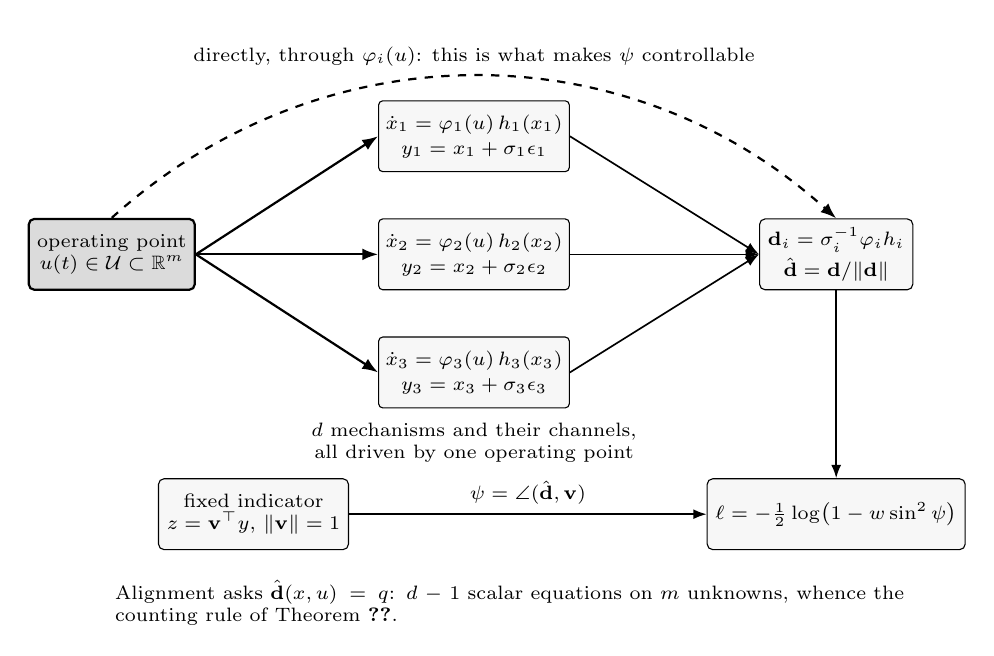
\begin{tikzpicture}[
  font=\small,
  b/.style={draw, rounded corners=1.5pt, align=center, inner sep=2.5pt,
            minimum height=9mm, fill=black!3, font=\scriptsize},
  lev/.style={draw, rounded corners=2pt, align=center, inner sep=3pt,
              minimum height=9mm, fill=black!14, thick, font=\scriptsize},
  ob/.style={draw, rounded corners=2pt, align=center, inner sep=3pt,
             minimum height=9mm, fill=black!3, font=\scriptsize},
  a/.style={-{Latex[length=1.7mm]}, semithick},
  th/.style={-{Latex[length=2mm]}, thick},
  lbl/.style={font=\scriptsize, inner sep=1pt}]

% ---------------- the operating point ------------------------------------
\node[lev] (u) at (0,0) {operating point\\$u(t)\in\mathcal U\subset\R^{m}$};

% ---------------- the d mechanism tracks: dynamics and channel -----------
\foreach \i/\y in {1/15mm, 2/0mm, 3/-15mm} {
  \node[b] (m\i) at (46mm,\y)
        {$\dot x_{\i}=\varphi_{\i}(u)\,h_{\i}(x_{\i})$\\[1pt]
         $y_{\i}=x_{\i}+\sigma_{\i}\epsilon_{\i}$};
}
\foreach \i in {1,2,3} { \draw[th] (u.east) -- (m\i.west); }

\node[lbl, anchor=north, align=center] at (46mm,-21mm)
      {$d$ mechanisms and their channels,\\ all driven by one operating point};

% ---------------- whitening and the direction ----------------------------
\node[ob] (d) at (92mm,0)
      {$\dvec_i=\sigma_i^{-1}\varphi_i h_i$\\[1pt]$\dhat=\dvec/\|\dvec\|$};
\foreach \i in {1,2,3} { \draw[a] (m\i.east) -- (d.west); }

% ---------------- indicator, angle, loss ---------------------------------
\node[ob] (v) at (18mm,-33mm)
      {fixed indicator\\$z=\mathbf v^{\top}y$, $\|\mathbf v\|=1$};
\node[ob] (l) at (92mm,-33mm)
      {$\lloss=-\tfrac12\log\!\big(1-w\sin^{2}\psi\big)$};

\draw[a] (d) -- (l);
\draw[a] (v) -- node[above, font=\scriptsize]
      {$\psi=\angle(\dhat,\mathbf v)$} (l);

% ---------------- the second path ----------------------------------------
\draw[th, dashed] (u.north) to[out=42, in=138]
      node[above, font=\scriptsize]
      {directly, through $\varphi_i(u)$: this is what makes $\psi$ controllable}
      (d.north);

\node[lbl, align=left, anchor=north west, text width=105mm] at (0mm,-41mm)
      {Alignment asks $\dhat(x,u)=q$: $d-1$ scalar equations on $m$ unknowns,
       whence the counting rule of Theorem~\ref{thm:zero}.};
\end{tikzpicture}
\caption{The construction. The operating point enters twice, through the plant and directly through $\varphi_i(u)$; the second path is what makes the misalignment $\psi$ a control variable. One input drives all $d$ mechanisms.}
\label{fig:framework}
\end{figure*}

Because $R$ is scalar, a single signal-to-noise ratio governs the information
the record carries about it, namely the squared sensitivity times the prior
uncertainty,
\begin{equation}
\gamma=\|\dvec\|^{2}\,\Var[R].
\label{eq:gamma}
\end{equation}

Rates in \eqref{eq:dvec} are taken with respect to clock time,
whereas~\cite{le2026jestech} differentiates with respect to age normalised by
$T_f$. The two conventions differ by a factor common to all $d$ channels, so
they give the same $\dhat$, and hence the same geometry in
Sections~\ref{sec:simplex}--\ref{sec:reach}, while rescaling $\gamma$.
Section~\ref{sec:limit}, where lifetime enters the objective, restores the
normalised convention.

\subsection{The fixed health indicator and its information loss}

A health indicator compresses the $d$ measured channels into one scalar before
any life prediction is made. We take it to be a fixed linear map. Since \eqref{eq:dvec} already measures each channel in units of its own noise, we write the indicator in those same coordinates: with $\Sigma:=\mathrm{diag}(\sigma_1^{2},\dots,\sigma_d^{2})$ and $\tilde y:=\Sigma^{-1/2}y$ the whitened record,
\begin{equation}
z=\mathbf v^{\top}\tilde y,\qquad \|\mathbf v\|=1,
\label{eq:hi}
\end{equation}
with the weight vector $\mathbf v$ chosen once, at design time, and held for
the whole life of the component. Fixing it is not a modelling convenience: the
map is typically embedded in firmware or frozen by certification, so it cannot be re-tuned as the component ages. An indicator specified on the raw measurements, $z=\mathbf w^{\top}y$, is the same map under $\mathbf v\propto\Sigma^{1/2}\mathbf w$, and the normalisation $\|\mathbf v\|=1$ only fixes the scale of $z$; it restricts nothing. The distinction matters because the angle below is measured after whitening: unless the $\sigma_i$ are equal, a unit vector in raw coordinates is not a unit vector in whitened ones, and the two readings of $\psi$ disagree.

We compute the cost of fixing $\mathbf v$ as follows. Write $\psi(t)$ for the
angle between the informative direction $\dhat(t)$ and the indicator weights
$\mathbf v$. After whitening, the signal in the record points along $\dhat$
and has magnitude $\|\dvec\|\sqrt{\Var[R]}$, while the noise is isotropic of
unit scale. Projecting onto a unit vector $\mathbf v$ therefore keeps the
fraction $\cos\psi$ of the signal and all of the noise, so the indicator's
signal-to-noise ratio is
\begin{equation}
\gamma\cos^{2}\psi
\label{eq:snrhi}
\end{equation}
against the $\gamma$ of \eqref{eq:gamma} available to an oracle that is free
to re-aim its projection at $\dhat(t)$ at every instant. Since a scalar
Gaussian channel of signal-to-noise ratio $s$ carries $\tfrac12\log(1+s)$ nats
about $R$~\cite{cover2006}, the information the fixed indicator forfeits, at
each instant, is
\begin{equation}
\lloss=\tfrac12\big[\log(1+\gamma)-\log(1+\gamma\cos^{2}\psi)\big]\ \ \ge 0 ,
\label{eq:lossraw}
\end{equation}
The design objective throughout is its average over the life of the component,
\begin{equation}
\bar\lloss:=\frac{1}{T_f}\int_{0}^{T_f}\lloss(t)\,dt ,
\label{eq:objective}
\end{equation}
a loss per unit time. We optimise this rate rather than the information the whole observation record forfeits, because \eqref{eq:objective} is unaffected by how densely the record is sampled and is therefore a property of the indicator rather than of the measurement schedule. The two are different quantities, and Proposition~\ref{prop:record} gives the second in closed form.

A third quantity is the one an operator actually pays for: the error of whatever remaining-life estimator runs downstream. It is neither of the first two and is not a function of them. The loss is a logarithmic information quantity and the error is a time, and an estimator holding a whole history recovers much of what any single instant discards, so a large spread in \eqref{eq:objective} does not imply a comparable spread in error. What the theory can offer downstream is therefore an ordering rather than a conversion, and Section~\ref{sec:downstream} tests that ordering against an estimator built from none of this construction: it survives, with a spread in error much smaller than the spread in loss. Equation~\eqref{eq:objective} should be read accordingly, as an information-geometric objective whose ranking carries downstream, not as a surrogate for prognostic accuracy.

Two remarks on what \eqref{eq:lossraw} does and does not say. It is a loss
relative to an oracle that no fixed map can realise, so it measures the price
of the time-invariance constraint rather than of a bad design; a perfectly
chosen $\mathbf v$ still pays it whenever $\dhat$ moves. And it depends on the
indicator only through the single angle $\psi$: two indicators that make the
same angle with $\dhat$ are equally good, whatever else distinguishes them.

The next lemma replaces \eqref{eq:lossraw} by a closed form that will be more
convenient throughout, and records how it behaves at small misalignment.

\begin{lemma}\label{lem:exact}
Let $w:=\gamma/(1+\gamma)\in(0,1)$. Then
\begin{equation}
\lloss=-\tfrac12\log\!\big(1-w\sin^{2}\psi\big),
\label{eq:exact}
\end{equation}
exactly and at every signal-to-noise ratio, and
\begin{equation}
\lloss=\tfrac{w}{2}\psi^{2}+\tfrac{w(3w-2)}{12}\psi^{4}+O(\psi^{6}).
\label{eq:expansion}
\end{equation}
\end{lemma}

\begin{proof}
Substituting $\cos^{2}\psi=1-\sin^{2}\psi$ into \eqref{eq:lossraw} gives
\[
\lloss=-\tfrac12\log\frac{1+\gamma-\gamma\sin^{2}\psi}{1+\gamma}
=-\tfrac12\log\big(1-w\sin^{2}\psi\big).
\]
For \eqref{eq:expansion}, use
$-\tfrac12\log(1-s)=\tfrac{s}{2}+\tfrac{s^{2}}{4} +O(s^{3})$ with
$s=w\sin^{2}\psi$ and $\sin^{2}\psi=\psi^{2}-\psi^{4}/3+O(\psi^{6})$;
collecting the $\psi^{4}$ terms gives $-w/6+w^{2}/4=w(3w-2)/12$.
\end{proof}

The quadratic term of \eqref{eq:expansion} is the bound obtained in
\cite[Thm.~1]{le2026jestech}, which is therefore the leading term of an exact
identity rather than an approximation of unknown quality. The quartic
coefficient $w(3w-2)/12$ changes sign at $w=2/3$, that is at $\gamma=2$: below
that signal-to-noise ratio the quadratic model overstates the loss, above it
the model understates it. This matters in practice because prognostic problems
sit on both sides of $\gamma=2$: an early-life measurement with a weak signal
on one side, a well-instrumented component near failure on the other.
Fig.~\ref{fig:mech}(a) plots the exact loss against its quadratic
approximation on both sides of that ratio.


\begin{proposition}\label{prop:record}
Let the record consist of measurements \eqref{eq:obs} at instants $t_1,\dots,t_N$, with the noise independent across channels and across instants, and write $\dvec_k:=\dvec(t_k)$ and $\psi_k$ for the angle between $\dhat_k$ and $\mathbf v$. Put
\begin{gather*}
G:=\Var[R]\sum_{k=1}^{N}\|\dvec_k\|^{2},\qquad
W:=\frac{G}{1+G},\\
S:=\frac{\sum_{k}\|\dvec_k\|^{2}\sin^{2}\psi_k}{\sum_{k}\|\dvec_k\|^{2}} .
\end{gather*}
Then the information about $R$ that the fixed indicator forfeits over the whole record is
\begin{equation}
\lloss_{\mathrm{rec}}=-\tfrac12\log\big(1-W S\big).
\label{eq:record}
\end{equation}
\end{proposition}

\begin{proof}
See Supplementary Section~S2.
\end{proof}

Equation \eqref{eq:record} is \eqref{eq:exact} again, with the instantaneous signal-to-noise ratio $\gamma$ replaced by its sum $G$ over the record, and $\sin^{2}\psi$ by the mean $S$ weighted by the signal energy $\|\dvec_k\|^{2}$. The reduction to one angle therefore survives the passage from an instant to a record. What does not survive is the averaging: $\bar\lloss$ averages the loss, whereas \eqref{eq:record} averages $\sin^{2}\psi$ inside it, and the two differ. They also select different indicators. Minimising \eqref{eq:record} over $\|\mathbf v\|=1$ maximises $\mathbf v^{\top}\big(\sum_k\dvec_k\dvec_k^{\top}\big)\mathbf v$, so the best fixed indicator for the record is the leading eigenvector of the integrated Fisher matrix, while the minimiser of $\bar\lloss$ is the barycentre of Proposition~\ref{prop:bary}. Every result below is stated for $\bar\lloss$.

\begin{corollary}[what the loss costs an estimator]\label{cor:mmse}
In the model of Section~\ref{sec:prelim}, the minimum-variance estimate of $R$ formed from the fixed indicator carries mean-squared error
\[
\frac{\Var[R\mid z]}{\Var[R\mid\tilde y]}=\frac{1+\gamma}{1+\gamma\cos^{2}\psi}=e^{2\lloss}
\]
times that of the estimate formed from the whole whitened record, at each instant. The same identity holds over a record with $\lloss$ replaced by $\lloss_{\mathrm{rec}}$ of Proposition~\ref{prop:record}.
\end{corollary}

\begin{proof}
Write $\tilde y=\dvec R+\epsilon$ with $\epsilon\sim N(0,I_d)$ and $R$ Gaussian. The indicator returns $z=(\mathbf v^{\top}\dvec)R+\mathbf v^{\top}\epsilon$, whose noise is standard normal because $\|\mathbf v\|=1$, so its signal-to-noise ratio is $\gamma\cos^{2}\psi$ and $\Var[R\mid z]=\Var[R]/(1+\gamma\cos^{2}\psi)$. The record's sufficient statistic is $\dvec^{\top}\tilde y$, with ratio $\gamma$, giving $\Var[R\mid\tilde y]=\Var[R]/(1+\gamma)$. Their quotient is $e^{2\lloss}$ by \eqref{eq:lossraw}. The record statement is the same computation with $G$ and $S$ in place of $\gamma$ and $\sin^{2}\psi$.
\end{proof}

The loss is therefore not a score standing in for estimation error: it is the logarithm of the factor by which that error inflates. What the corollary does not settle is whether the ordering survives an estimator other than the one the model prescribes, and Section~\ref{sec:downstream} checks that separately.


\begin{figure}[t]
\centering 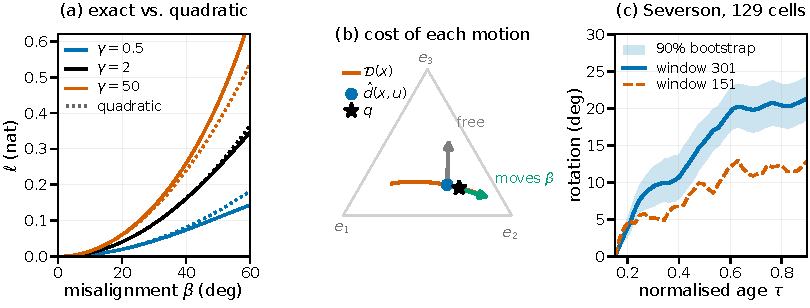
\includegraphics[width=\linewidth]{fig2.pdf}
\caption{(a)~Lemma~\ref{lem:exact}: the exact loss (solid) against its quadratic model (dotted), whose quartic coefficient changes sign at $\gamma=2$. (b)~Theorem~\ref{thm:beta}: of the replicator velocity, only the component along the geodesic towards $q$ moves $\beta$. (c)~The rotation, measured on the Severson fleet at two differentiation windows.}
\label{fig:mech}
\end{figure}

\section{The information simplex and its replicator flow}
\label{sec:simplex}

Lemma~\ref{lem:exact} reduced the loss to one angle. This section shows that
the angle lives on a familiar object, the probability simplex, and that the
degradation traces a flow along it that the operating point drives. The payoff is threefold: the loss becomes a recognised statistical distance, the optimal indicator becomes a barycentre, and the effect of the input becomes a single interpretable quantity. Two of the results here are load-bearing for what follows --- the replicator form of Theorem~\ref{thm:repl} and the misalignment rate of Theorem~\ref{thm:beta}, which Section~\ref{sec:reach} builds the reachability argument on. The Bhattacharyya identity and the barycentre are interpretation: they say what the loss and the optimal indicator already are in recognised terms, and nothing later depends on them.

\subsection{Information shares}

Because every entry of $\dvec$ is positive (Section~\ref{sec:dvec}), the
squared components of the unit vector $\dhat$ form a probability vector:
\begin{equation}
p_i:=\dhat_i^{2},\qquad p_i>0,\qquad \textstyle\sum_i p_i=1 .
\label{eq:shares}
\end{equation}
The interpretation is direct. The total Fisher information the record carries
about $R$ is $\|\dvec\|^{2}\Var[R]$ by \eqref{eq:gamma}, and channel $i$
contributes $\dvec_i^{2}\Var[R]$ of it. So $p_i$ is exactly the share of the
total information about remaining life that arrives through channel $i$. A
component in which one mechanism dominates the degradation has $p$ near a
vertex of the simplex; one in which three mechanisms contribute equally sits
near its centre.

The same map applied to the indicator, $q_i:=\mathbf v_i^{2}$, is legitimate
because an optimal indicator may be taken with non-negative weights.

\begin{remark}[positivity is load-bearing]\label{rem:pos}
If $\dhat\ge0$ then $\dhat^{\top}|\mathbf v|\ge|\dhat^{\top}\mathbf v|$ at
every instant, so replacing $\mathbf v$ by $|\mathbf v|$ never increases
\eqref{eq:lossraw}: non-negative weights are without loss of generality. This
argument uses the positivity of $\dvec$ inherited from $\varphi_i,h_i>0$, and
it fails without it: in random trials with sign-indefinite $\dhat$, taking
absolute values was worse than the signed vector about a third of the time.
The results therefore require the positive-orthant structure of the
degradation model; it is not only a notational convenience.
\end{remark}

\subsection{The loss as a Bhattacharyya distance}

The identification below is used twice in what follows: it gives ``the average
of a curve on the simplex'' an unambiguous meaning (Section~\ref{sec:bary}),
and it lets the high-signal limit of the loss be read off as a known
divergence.

\begin{proposition}\label{prop:bhat}
$\cos\psi=\sum_i\sqrt{p_iq_i}$ is the Bhattacharyya coefficient of $p$ and
$q$. Consequently $\psi=\tfrac12\dFR(p,q)$, where $\dFR$ is the Fisher--Rao
distance on the simplex, and, writing $\DB(p,q)=-\log\sum_i\sqrt{p_iq_i}$ for
the Bhattacharyya divergence,
\begin{equation}
\lloss=-\tfrac12\log\!\big[(1-w)+w\,e^{-2\DB(p,q)}\big].
\label{eq:bhat}
\end{equation}
As $\gamma\to\infty$, $\lloss\to\DB(p,q)$.
\end{proposition}

\begin{proof}
By construction,
\[
\cos\psi=\dhat^{\top}\mathbf v=\sum_i\sqrt{p_i}\sqrt{q_i},
\]
which is precisely the Bhattacharyya coefficient of $p$ and $q$. The map
$p\mapsto\sqrt p$ is the classical isometry between the simplex under the
Fisher--Rao metric and the positive orthant of the unit sphere, under which
the geodesic distance is twice the spherical
angle~\cite{amari2016,bhattacharyya1943}; hence $\psi=\tfrac12\dFR$. Then
$\cos^{2}\psi=e^{-2\DB}$, and substituting into \eqref{eq:exact} gives
\eqref{eq:bhat}. Letting $w\to1$ gives the limit.
\end{proof}

The square root is a bijection between the simplex and the non-negative part
of the unit sphere, carrying $p$ to $\dhat$ and $q$ to $\mathbf v$, and by the
proposition it is an isometry. We use the two descriptions interchangeably
from here on: a statement such as $q\in\mathcal D(x)$ in
Section~\ref{sec:reach} says that $\mathbf v$ is a reachable direction, and a
distance between points of the simplex is the angle between the corresponding
unit vectors.

The resulting picture is the one the rest of the paper develops. The degrading
component is a curve on the simplex, the health indicator is a single point on
it, and the information lost depends only on the distance between them. Design
of the indicator is the choice of one point; control of the operating point is
the shaping of the curve.

\subsection{The optimal indicator as a barycentre}
\label{sec:bary}

If the indicator is one point and the plant is a curve, the best point should
be some kind of average of the curve. It is, but of two different kinds in two
different limits.

\begin{proposition}\label{prop:bary}
Let $q^{\star}$ minimise the time-averaged loss.
\begin{enumerate}
\item[(i)] As $\gamma\to\infty$, $\lloss\to\DB$ pointwise, so $q^{\star}$
tends to the Bhattacharyya barycentre $\arg\min_q\int\DB(p_\tau,q)\,d\tau$.
\item[(ii)] As the curve shortens, $\lloss=\tfrac{w}{2}\psi^{2}+O(\psi^{4})$,
so $q^{\star}$ tends to the $w$-weighted Fisher--Rao barycentre, and
$\bar\lloss=\tfrac18\bar w\,\mathrm{Var}^{\mathrm{FR}}+O(\psi^{4})$ where
$\mathrm{Var}^{\mathrm{FR}}:=\min_q\E_\mu[\dFR^{2}(p_\tau,q)]$ is the
$\mu$-weighted Fr\'echet variance of the curve.
\end{enumerate}
\end{proposition}

\begin{proof}
See Supplementary Section~S2.
\end{proof}

The two limits are taken in different parameters, signal-to-noise ratio in (i)
and arc length in (ii), and they do not coincide. On a curve of angular span
$82.7^{\circ}$ the two barycentres lie $0.72^{\circ}$ apart, and $q^{\star}$
crosses from the Fisher--Rao side to the Bhattacharyya side between $0$ and
$10$~dB, reaching $3\times10^{-5}$ degrees of the latter by $50$~dB. For
design purposes the practical consequence is mild: either barycentre of a
nominal degradation path is a good starting indicator.

\subsection{The replicator flow and the role of the input}

We now ask how fast the informative direction moves and what the operating
point does to that motion.

\begin{theorem}\label{thm:repl}
Let $g_i=\log\dvec_i$ denote the logarithmic rate of channel $i$. Along
\eqref{eq:plant},
\begin{equation}
\dot{\dhat}_i=\dhat_i\big(\dot g_i-\E_p[\dot g]\big),
\label{eq:dhatdot}
\end{equation}
so the information shares obey the replicator equation of evolutionary
dynamics, in which each share grows in proportion to the amount by which its
own rate exceeds the average, the average being taken over the shares
themselves:
\begin{equation}
\dot p_i=2p_i\big(\dot g_i-\E_p[\dot g]\big),
\label{eq:replicator}
\end{equation}
and
\begin{equation}
\|\dot{\dhat}\|=\Std_p[\dot g],\qquad \dot g=\big[\varphi_i(u)h_i'(x_i)\big]_i
+\,\nabla_{\!u}\!\log\varphi\;\dot u .
\label{eq:repl}
\end{equation}
\end{theorem}

\begin{proof}
From $\dvec_i=e^{g_i}$ we have $\dot\dvec_i=\dvec_i\dot g_i$, so
$\dot{\dhat}=\|\dvec\|^{-1}\big(\dot\dvec-\dhat(\dhat^{\top}\dot\dvec)\big)$
has components $\dhat_i\dot g_i-\dhat_i\sum_j\dhat_j^{2}\dot g_j$, which is
\eqref{eq:dhatdot}; squaring and summing gives $\Var_p[\dot g]$. Since
$p_i=\dhat_i^{2}$, $\dot p_i=2\dhat_i\dot{\dhat}_i=2p_i(\dot g_i-\E_p[\dot
g])$. Differentiating $g_i=\log\varphi_i(u)+\log h_i(x_i)-\log\sigma_i$ along
\eqref{eq:plant} gives $\dot g_i=\nabla_{\!u}\log\varphi_i\cdot\dot
u+(h_i'/h_i)\varphi_ih_i$, and $(h_i'/h_i)\varphi_ih_i=\varphi_ih_i'$.
\end{proof}

Equation \eqref{eq:repl} has a compact reading. The speed at which the
informative direction rotates equals the information-weighted spread of the
mechanisms' logarithmic rates. If all mechanisms accelerate at the same
proportional rate the direction does not move at all, however fast the
component is degrading; it is disagreement among the mechanisms that rotates
it. The identity is the Fisher--Rao/Shahshahani geometry of the simplex
combined with Fisher's fundamental theorem of natural
selection~\cite{amari2016,hofbauer1998,sandholm2010}. What is new here is its
identification with the informative direction of a degrading component, and,
decisively, that the quantity playing the role of fitness, the logarithmic
rate $\dot g_i$ of channel $i$, is actuated: the second summand in
\eqref{eq:repl} is the operator's lever.

\begin{remark}[contrast with Oja's flow]
Oja's flow for online principal-component extraction has the same algebraic
form; for a diagonal covariance it reduces to a replicator equation with
fitness twice the eigenvalues~\cite{oja1982}. The roles are opposite. There
the flow is an algorithm, run to fixation in order to find a direction, with
constant fitness. Here it is the plant, its fitness is time-varying and
actuated, and the aim is to prevent fixation from carrying the direction away
from a fixed indicator.
\end{remark}

Only one scalar matters for the loss. Fix the indicator $q$ and write
$\beta:=\angle(\dhat,\mathbf v)=\tfrac12\dFR(p,q)$ for the misalignment. This
is the angle $\psi$ of Lemma~\ref{lem:exact} under a new name, and the change
of name marks a change of role: $\psi$ was a fixed angle between two
directions, whereas $\beta=\beta(x_t,u_t)$ is followed along the trajectory
and is the quantity the input acts on. Every loss expression below may
therefore be read as a function of $\beta$.

\begin{theorem}\label{thm:beta}
Let the operating-point trajectory $u(\cdot)$ be absolutely continuous, and let $\hat e$ be the unit tangent at $\dhat$ along the geodesic towards $\mathbf v$. Then $\dot\beta=-\langle\dot{\dhat},\hat e\rangle$, which is
affine in the input rate: $\dot\beta=\alpha_0(x,u)+\alpha(x,u)^{\top}\dot u$.
In particular $|\dot\beta|\le\|\dot{\dhat}\|$, with equality only for motion
along that geodesic.
\end{theorem}

\begin{proof}
$\cos\beta=\dhat^{\top}\mathbf v$ gives
$-\sin\beta\,\dot\beta=\dot{\dhat}^{\top}\mathbf v$. Also $\hat e=(\mathbf
v-\cos\beta\,\dhat)/\sin\beta$ and $\dot{\dhat}^{\top}\dhat=0$, so
$\langle\dot{\dhat},\hat e\rangle=\dot{\dhat}^{\top}\mathbf v/\sin\beta
=-\dot\beta$. Affinity follows because $\dot g$ is affine in $\dot u$ by
\eqref{eq:repl} and $\dot{\dhat}$ is linear in $\dot g$.
\end{proof}

The hypothesis is needed only to write $\dot u$; nothing in Section~\ref{sec:reach} depends on it, since the reachable sets \eqref{eq:reachset} are defined pointwise in $u$ and the limits below hold for every measurable admissible input. Theorem~\ref{thm:beta} is a local kinematic description of smooth steering, not a restriction on the controls the rest of the paper admits.

The component of the replicator velocity orthogonal to $\hat e$ is therefore free: the informative direction may rotate in a $(d-2)$-dimensional subspace
at no cost in information. Fig.~\ref{fig:mech}(b) shows the decomposition at
one state. This is the observation that separates the two objectives of the
next section.

\section{Reachability limits on the misalignment}
\label{sec:reach}

Controlling the rate $\dot\beta$ is not the same as reaching a value of
$\beta$. The distinction is the subject of this section, and it is what
decides whether a fixed indicator can be made lossless at all.

For a state $x$, the set of informative directions the operator can produce by
choosing the operating point is
\begin{equation}
\mathcal D(x):=\{\dhat(x,u):u\in\mathcal U\}\subset S^{d-1},
\label{eq:reachset}
\end{equation}
the reachable direction set, and the closest the indicator can be brought at
that state is the reachable misalignment floor
\begin{equation}
\beta_{\min}(x,q):=\mathrm{dist}\big(q,\mathcal D(x)\big).
\label{eq:floor}
\end{equation}
For a single input, $\mathcal D(x)$ is an arc traced out as $u$ sweeps
$\mathcal U$; its length measures the actuation authority available at $x$,
and it shrinks to a point when the mechanisms respond identically to the
input.

\begin{theorem}\label{thm:zero}
Fix an admissible input and let $x(\cdot)$ be the trajectory it generates. Zero loss along that trajectory is attainable with the fixed indicator $q$ if and only if $q\in\bigcap_{t}\mathcal D(x_t)$. If $m<d-1$ and $u\mapsto\dhat(x,u)$ is continuously differentiable, the indicators that attain zero loss form a null subset of the unit sphere, so almost every $q$, and in fact every $q$ that does not attain it, has $\beta_{\min}>0$ on a set of times of positive measure. Whether any $q$ at all attains zero loss is a property of the plant, and Remark~\ref{rem:family} exhibits plants for which one does. In every case
$\bar{\lloss}\ge\int\lloss(\beta_{\min}(x_t,q))\,dt/T_f$ for that trajectory.
\end{theorem}

\begin{proof}
By Lemma~\ref{lem:exact}, $\lloss(\beta)=0$ iff $\sin\beta=0$, so
$\bar\lloss=0$ iff $\beta_t=0$ for almost every $t$, that is iff
$\dhat(x_t,u_t)=q$, that is iff $q\in\mathcal D(x_t)$ for every $t$. Solving
$\dhat(x,u)=q$ imposes $d-1$ independent scalar equations, both sides being
unit vectors, on $m$ unknowns. If $m<d-1$ then $\mathcal D(x)$, the image of an $m$-dimensional set under a continuously differentiable map, is a null subset of the $(d-1)$-dimensional sphere, which almost every $q$ misses; if $m\ge d-1$ the
implicit function theorem supplies a solution wherever the Jacobian has full
rank. The inequality $\beta_t\ge\beta_{\min}(x_t,q)$ holds for every
admissible input by definition of $\beta_{\min}$ as a minimum over $\mathcal
U$, and is strict exactly where $q\notin\mathcal D(x_t)$. Since $\mathcal U$ is compact and $\dhat$ continuous, each $\mathcal D(x_t)$ is compact and varies continuously with $t$, so the set of times at which $q\notin\mathcal D(x_t)$ is open. It is non-empty for every $q$ that does not attain zero loss, in particular for every $q$ outside the null set $\mathcal D(x_0)$, and so has positive measure. Since $\lloss$ is increasing on $[0,\pi/2]$, the bound follows on
dividing by $T_f$.
\end{proof}

This is a state-conditioned result. The bound is genuine, in the sense that no input violates a reachability constraint at the state it occupies, but it is conditional on the trajectory, which the input also steers. Optimising over the trajectory as well is deferred to Section~\ref{sec:limit}, and the two levels are the structure of the argument: a state-conditioned limit here, a trajectory-level limit there.

The practical reading of Theorem~\ref{thm:zero} is a counting rule: a
component degrading through $d$ mechanisms generically needs $d-1$
independently adjustable operating variables before a fixed indicator can be
kept perfectly aligned. Here \emph{generically} is a count of dimensions over the plant's data, not a statement of measure: the theorem proves the measure statement over indicators, Remark~\ref{rem:family} constructs plants that escape the count, and we do not prove those plants rare. Section~\ref{sec:translate} says what the qualifier covers. For a generic plant under this model, three mechanisms and a single temperature setpoint will not do it. The three results of this section answer different questions, and it is worth separating them. Theorem~\ref{thm:zero} characterises zero loss exactly, as membership of every reachable set, and then counts dimensions to say when a generic plant can meet it; the count is necessary for generic data and is not by itself a construction. Proposition~\ref{prop:contain} gives an exact criterion, necessary and sufficient, on the separable subclass alone. Remark~\ref{rem:family} exhibits plants outside that subclass which attain zero loss with fewer inputs than the count asks, so the count is not necessary in general. But a weaker and much cheaper objective is available.

\begin{corollary}[what actuation is actually required]\label{cor:tri}
Two objectives that are easily conflated carry different requirements.
\begin{enumerate}
\item[(i)] Driving $\bar\lloss$ to zero is equivalent to freezing $\dhat$ at
  $q$, and needs $d-1$ conditions on $\dot u$, hence generically $m\ge d-1$.
\item[(ii)] Holding $\beta$ at a constant level, not necessarily zero, is
the single scalar equation $\alpha_0+\alpha^{\top}\dot u=0$, solvable whenever
$\alpha\ne0$ and the resulting $u(\cdot)$ stays in $\mathcal U$; generically
$m\ge1$ suffices.
\end{enumerate}
\end{corollary}

\begin{proof}
(i) By Theorem~\ref{thm:zero}, $\bar\lloss=0$ iff $\dhat(x_t,u_t)=q$ for every
$t$, so $\dhat$ is constant; by Theorem~\ref{thm:repl} that forces $\dot
g_i=\E_p[\dot g]$ for every $i$, which is $d-1$ independent conditions on
$\dot u\in\R^{m}$. (ii) is one equation in $\dot u$ by Theorem~\ref{thm:beta}.
The gap between them is the content of that theorem: $\dot\beta$ sees only the
component of $\dot{\dhat}$ along $\hat e$, so the remaining $d-2$ directions
of rotation are unconstrained by (ii) and constrained by (i).
\end{proof}

Minimising $\bar\lloss$ is neither of these: it trades the level of $\beta$
against the trajectory that carries it, and is the problem of
Section~\ref{sec:limit}.

\subsection{The reachable sets are translates of one set}
\label{sec:translate}

Theorem~\ref{thm:zero} counts equations against unknowns and hedges with
``generic''. The hedge is not idle, and the following observation says exactly
what it covers.

\begin{lemma}[separability]\label{lem:sep}
Write $\xi(x,u)$ for the class of $\log\dvec(x,u)$ modulo the all-ones vector,
which is what $\dhat$ retains. Then
\begin{equation}
\begin{aligned}
\xi(x,u) &= a(x)+b(u),\\
a_i(x) &= \log\frac{h_i(x_i)}{\sigma_i},\qquad
b_i(u) = \log\varphi_i(u),
\end{aligned}
\label{eq:sep}
\end{equation}
both taken modulo the all-ones vector. Consequently every reachable direction
set is the same set translated: $\mathcal D(x)=a(x)+\mathcal B$ with $\mathcal
B:=b(\mathcal U)$ fixed.
\end{lemma}

\begin{proof}
Immediate from $\dvec_i=\sigma_i^{-1}\varphi_i(u)h_i(x_i)$ in \eqref{eq:dvec}:
the logarithm turns the product into a sum, and the normalisation of $\dhat$
removes any component along the all-ones vector.
\end{proof}

The decomposition separates the two parties. The set $\mathcal B$ is fixed by the stress model $\varphi$ and the envelope $\mathcal U$ alone (Fig.~\ref{fig:sep}(a)). An operator's authority can therefore be computed offline from the accelerated-life model, with no degradation record at all. The curve $\mathcal A:=\{a(x_t)\}$ is fixed by the damage shapes $h$ and the noise levels $\sigma$, and every reachable set is that one set carried along it (Fig.~\ref{fig:sep}(b)). What the geometry of Section~\ref{sec:simplex} measures is how far
the plant's demand $\mathcal A$ sticks out of the operator's authority
$\mathcal B$.

That offline route is the most useful consequence drawn in this paper and also
the most restrictive. It holds on the separable subclass and not beyond it,
and the best high-fidelity turbofan data we have reject separability
(Section~\ref{sec:scope}). This subsection and Proposition~\ref{prop:contain}
should therefore be read as describing a structured subclass that is
convenient when it applies, not as a general account of real machinery.
Fig.~\ref{fig:scope} marks the one branch of the development that depends on it.


\begin{figure*}[tb]
\centering
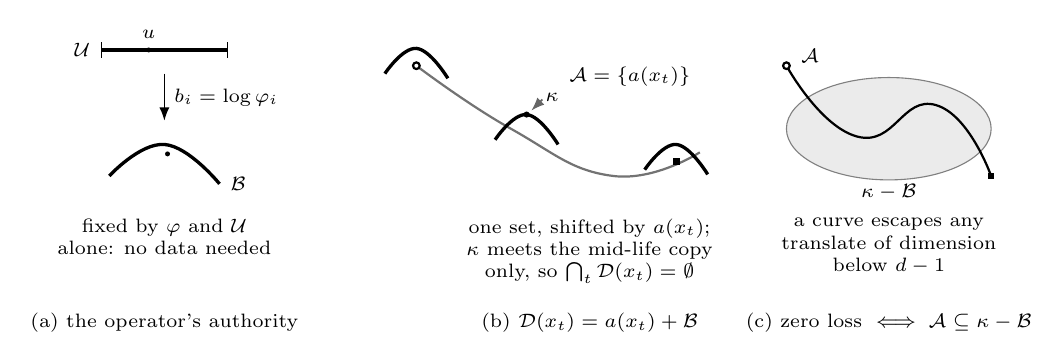
\begin{tikzpicture}[
  font=\small,
  auth/.style={very thick},
  crv/.style={thick},
  a/.style={-{Latex[length=1.7mm]}, semithick},
  lbl/.style={font=\scriptsize, inner sep=1pt},
  cp/.style={font=\scriptsize, align=center, inner sep=1pt}]

% =================== (a) the authority set is built from U ===============
\begin{scope}
  % the admissible input set
  \draw[very thick] (0,12mm) -- (16mm,12mm);
  \foreach \x in {0,16mm} { \draw (\x,11mm) -- (\x,13mm); }
  \node[lbl, anchor=east] at (-1mm,12mm) {$\mathcal U$};
  \fill (6mm,12mm) circle (0.9pt);
  \node[lbl, anchor=south] at (6mm,13mm) {$u$};

  \draw[a] (8mm,9mm) -- node[right, font=\scriptsize]
        {$b_i=\log\varphi_i$} (8mm,3mm);

  \draw[auth] plot[smooth, tension=0.8] coordinates
      {(1mm,-4mm) (8mm,0mm) (15mm,-5mm)};
  \fill (8.4mm,-1.2mm) circle (0.9pt);
  \node[lbl, anchor=west] at (16mm,-5mm) {$\mathcal B$};

  \node[cp, anchor=north] at (8mm,-9mm)
        {fixed by $\varphi$ and $\mathcal U$\\alone: no data needed};
  \node[cp, anchor=north] at (8mm,-21mm) {(a) the operator's authority};
\end{scope}

% =================== (b) every reachable set is that set, translated =====
\begin{scope}[xshift=40mm]
  \draw[crv, black!55] plot[smooth, tension=0.8] coordinates
      {(0mm,10mm) (12mm,2mm) (25mm,-4mm) (36mm,-1mm)};
  \node[lbl, anchor=south west] at (19mm,7mm) {$\mathcal A=\{a(x_t)\}$};

  \foreach \sx/\sy in {0mm/10mm, 14mm/1.6mm, 33mm/-2.2mm} {
    \begin{scope}[shift={(\sx,\sy)}]
      \draw[auth] plot[smooth, tension=0.8] coordinates
          {(-4mm,-1mm) (0mm,2.2mm) (4mm,-1.6mm)};
    \end{scope}
  }
  \draw[fill=white, thick] (0mm,10mm) circle (1.2pt);
  \fill (33mm,-2.2mm) +(-1.2pt,-1.2pt) rectangle +(1.2pt,1.2pt);

  \fill (14mm,3.8mm) circle (1.1pt);
  \node[lbl, anchor=west] at (16mm,6.0mm) {$\kappa$};
  \draw[a, black!60] (16mm,5.7mm) -- (14.6mm,4.3mm);

  \node[cp, anchor=north] at (22mm,-9mm)
        {one set, shifted by $a(x_t)$;\\
         $\kappa$ meets the mid-life copy\\
         only, so $\bigcap_t\mathcal D(x_t)=\emptyset$};
  \node[cp, anchor=north] at (22mm,-21mm)
        {(b) $\mathcal D(x_t)=a(x_t)+\mathcal B$};
\end{scope}

% =================== (c) the containment test ============================
\begin{scope}[xshift=86mm]
  \draw[fill=black!8, draw=black!50] (14mm,2mm) ellipse
      [x radius=13mm, y radius=6.5mm];
  \node[lbl] at (14mm,-6mm) {$\kappa-\mathcal B$};

  \draw[crv] plot[smooth, tension=0.9] coordinates
      {(1mm,10mm) (10mm,1mm) (20mm,5mm) (27mm,-4mm)};
  \draw[fill=white, thick] (1mm,10mm) circle (1.2pt);
  \fill (27mm,-4mm) +(-1.2pt,-1.2pt) rectangle +(1.2pt,1.2pt);
  \node[lbl, anchor=south] at (4mm,10mm) {$\mathcal A$};

  \node[cp, anchor=north] at (14mm,-9mm)
        {a curve escapes any\\
         translate of dimension\\
         below $d-1$};
  \node[cp, anchor=north] at (14mm,-21mm)
        {(c) zero loss $\iff\mathcal A\subseteq\kappa-\mathcal B$};
\end{scope}
\end{tikzpicture}
\caption{How the counting rule becomes a containment. (a)~The operator's authority $\mathcal B=b(\mathcal U)$, fixed by the stress model and the envelope alone. (b)~Every reachable set is that one set translated, $\mathcal D(x_t)=a(x_t)+\mathcal B$ (circle: start of life, square: failure). (c)~Zero loss asks the whole curve to lie in one translate (Proposition~\ref{prop:contain}).}
\label{fig:sep}
\end{figure*}

\begin{proposition}[exact criterion]\label{prop:contain}
Zero loss is attainable along a trajectory if and only if $\mathcal A$ is
contained in a translate of $-\mathcal B$. In particular $\mathcal A$ must lie
in an affine subspace of dimension at most $\dim \mathcal B\le m$, which for a
curve in the $(d-1)$-dimensional quotient fails generically unless $m\ge d-1$;
this recovers Theorem~\ref{thm:zero}. When it does not fail, $m<d-1$ suffices.
\end{proposition}

\begin{proof}
By Theorem~\ref{thm:zero}, zero loss holds iff $q\in\mathcal D(x_t)$ for every
$t$. Writing $\kappa$ for the quotient class of $\log\mathbf v$ and using
Lemma~\ref{lem:sep}, that reads $\kappa-a(x_t)\in \mathcal B$ for every $t$,
that is $\mathcal A\subseteq\kappa-\mathcal B$. The dimension statement
follows because a translate of $\mathcal B$ spans an affine subspace of
dimension $\dim \mathcal B$.
\end{proof}

The containment is drawn in Fig.~\ref{fig:sep}(c), and the mechanism the count obscures is now visible. Alignment at an instant fixes
$u_t$ outright, since $b(u_t)=\kappa-a(x_t)$ determines it; the input is
spent, and any residual constraint on the state must then hold along the flow
with no freedom left to enforce it. One input can carry the whole burden only
when no residual constraint is left, which happens when $\mathcal A$ already
lies parallel to $\mathcal B$.

\begin{remark}[a family with $m=1$ and any $d$]\label{rem:family}
Take exponential shapes $h_i(x)=e^{\nu_i(x_i-x_i^0)}$, which \eqref{eq:plant}
admits, and Arrhenius factors. Under the ramp $u(t)=u_0+rt$ the damage rates
are constant, $x_i(t)=x_i^0+\varphi_i^0t$ with $\varphi_i^0=\varphi_i(u_0)$,
so $a(x_t)$ moves at constant velocity $\nu_i\varphi_i^0$. Choosing
$\nu_i=rE_i/\varphi_i^0$ makes that velocity parallel to $E$, which is the
direction of $\mathcal B$, and $b(u_t)$ retreats along $\mathcal B$ at the
same rate. The two cancel and $\dhat$ is frozen. Supplementary Section~S4 integrates the construction for $d=2$ to $8$.
\end{remark}

This bears on the sharpness of Theorem~\ref{thm:zero}. The family of Remark~\ref{rem:family} is a knife
edge. At one percent of error in its shape coefficients, steering is already worse than not steering (Supplementary Section~S4). A designer should read
Proposition~\ref{prop:contain} as an explanation of when the counting rule
binds, and Theorem~\ref{thm:zero} as the rule to design against.

\subsection{Invisibility to Fisher-information criteria}

A natural objection is that all of this should follow from designing the input
to maximise the Fisher information about $R$, as in the observability-aware
literature discussed in Section~\ref{sec:intro}. It does not, and the reason
is structural.

\begin{proposition}[Fisher blindness]\label{prop:blind}
The loss of a fixed indicator is not a function of the Fisher information about $R$: configurations with equal Fisher information can have different losses, and configurations with equal losses can have different Fisher information. No criterion depending on the Fisher information alone can therefore rank fixed indicators by the loss they incur.
\end{proposition}

\begin{proof}
For a scalar latent the Fisher information is the number
$\|\dvec\|^{2}\Var[R]$, so trace, determinant and least eigenvalue coincide
and every scalarisation is a strictly monotone function of it. Under the
rescaling $\dvec\mapsto c\,\dvec$ with $c>0$, that number changes while
$\dhat$, and hence $\beta$ and $\lloss$, do not. A common gain therefore
equalises the scores of two configurations with different losses, and
separates the scores of two configurations with the same loss.
\end{proof}

Stated in engineering terms, a Fisher criterion measures the strength of the
signal, whereas the loss of a fixed indicator depends on its direction.
Amplifying every channel by the same factor increases the first and leaves the
second unchanged. Section~\ref{sec:num} exhibits this concretely: with the
Fisher score held equal to seven digits, the loss still spans a factor of
$9.4$.

\section{The best achievable loss as a fractional control problem}
\label{sec:limit}

Theorem~\ref{thm:zero} bounds the loss along a given trajectory. But the input
steers the trajectory as well as the misalignment on it, so the best achievable loss requires optimising over both at once. This changes the structure of the
problem.

The objective is a time average over a lifetime that the input itself
determines:
\begin{equation}
\bar{\lloss}^{\star}(q)=\min_{u(\cdot)\in\mathcal U}
\frac{\int_0^{T_f}\lloss(\beta(x_t,u_t))\,dt}{T_f}.
\label{eq:frac}
\end{equation}
Both the integrand and the upper limit $T_f$ depend on $u(\cdot)$. This makes
\eqref{eq:frac} a fractional optimal control problem, meaning that the
objective is a ratio rather than that the dynamics carry a fractional-order
derivative. The fraction is not a technicality: it is the source of the
trade-off, as follows.

Suppose $T_f$ were fixed. Nothing in \eqref{eq:plant} penalises the input
directly, so the answer would be trivial: find whichever admissible $u$ minimises $\beta$ and stay there. Because $T_f$ is itself controlled, the denominator of \eqref{eq:frac} rules that solution out. The
operating point that aligns the indicator is in general not the operating
point that prolongs life, so aligning now shortens the interval over which the
alignment is averaged. The optimum must trade the two, and
Section~\ref{sec:steer} measures how steep that trade is on a concrete plant.
A fixed-horizon formulation represents none of it, which is why one was tried
and discarded (Section~\ref{sec:steer}).

\subsection{A converse bound uniform over trajectories}
\label{sec:converse}

Before computing anything we record a certificate that removes the
conditioning. Theorem~\ref{thm:zero} bounds the loss along a trajectory the
input has already chosen; the following proposition bounds it over all of them
at once, and it is what would make the number computed below a limit rather than an observation, were a function satisfying it exhibited; none is, for reasons given below.

\begin{proposition}[verification certificate]\label{prop:converse}
Fix an indicator $q$ and a constant $\lambda\ge0$. Suppose there is a
continuously differentiable $V$ on a neighbourhood of the admissible state
region such that
\begin{enumerate}
\item[(i)] $V(x)\le0$ for every $x$ on the failure surface
  $\{\max_i x_i=1\}$, and
\item[(ii)] writing $D_i(x,u)=\varphi_i(u)h_i(x_i)$ for the drift of
\eqref{eq:plant}, for every admissible state $x$ and every $u\in\mathcal U$,
\begin{equation}
\lloss\big(\beta(x,u)\big)-\lambda+\nabla V(x)^{\top}D(x,u)\ \ge\ 0 .
\label{eq:cert}
\end{equation}
\end{enumerate}
Then every admissible input satisfies $\bar{\lloss}\ge\lambda+V(x_0)/T_f$. In
particular, if $V(x_0)\ge0$ then $\bar{\lloss}^{\star}(q)\ge\lambda$,
uniformly over all admissible inputs and hence over all trajectories.
\end{proposition}

\begin{proof}
Let $u(\cdot)$ be any admissible input and $x_t$ its trajectory. Since $V$ is
$C^{1}$ and $t\mapsto x_t$ is absolutely continuous, $t\mapsto V(x_t)$ is
absolutely continuous and the chain rule gives $\tfrac{d}{dt}V(x_t)=\nabla
V(x_t)^{\top}\dot x_t =\nabla V(x_t)^{\top}D(x_t,u_t)$ for almost every $t$.
Applying \eqref{eq:cert} at $(x_t,u_t)$ gives
$\lloss(\beta(x_t,u_t))-\lambda+\tfrac{d}{dt}V(x_t)\ge0$ a.e., and integrating
over $[0,T_f]$,
\[
\int_0^{T_f}\!\big(\lloss-\lambda\big)\,dt
\;\ge\;V(x_0)-V(x_{T_f})\;\ge\;V(x_0),
\]
the last step by (i), since $x_{T_f}$ lies on the failure surface. Dividing by
$T_f>0$ gives the claim.
\end{proof}

Condition \eqref{eq:cert} constrains the plant data alone: it quantifies over every state and every
admissible input, and mentions no trajectory. Any $V$ one can exhibit
therefore certifies a limit, and the search for a converse becomes the search
for a verification function.

The $C^{1}$ hypothesis is not a formality, and it is exactly what the
natural candidates lack: the value function of the Dinkelbach problem below is
only Lipschitz and violates \eqref{eq:cert} pointwise, while affine functions
are smooth but certify only a vacuous pointwise bound. Supplementary
Section~S3 records both attempts and what they imply, that a certificate must
be smooth and must have a gradient that varies, which points at a smooth
under-approximation of the value function by sum-of-squares programming or
interval arithmetic. We do not claim a certified converse here, and the optimum computed below remains a computation; what Proposition~\ref{prop:converse}
buys is the replacement of an open problem without shape by a concrete object
with a checkable property.

Problems of the form \eqref{eq:frac} are handled by Dinkelbach's
transform~\cite{dinkelbach1967}: setting
\begin{equation}
F(\lambda)=\min_{u(\cdot)\in\mathcal U}\int_0^{T_f}
\big(\lloss-\lambda\big)\,dt ,
\label{eq:dink}
\end{equation}
the map $F$ is decreasing in $\lambda$ and vanishes exactly at the optimal
ratio, so $\lambda^{\star}$ is found by bisection on $F(\lambda)=0$. The inner
problem in \eqref{eq:dink} has free terminal time and an absorbing set, hence
a stationary Hamilton--Jacobi--Bellman equation on the state alone, with no
time argument. Because $\dot x>0$ the state advances monotonically, and a
semi-Lagrangian scheme~\cite{falcone2014} converges by value iteration. One
implementation detail matters: the scheme must use a fixed spatial step rather
than a fixed time step, because degradation speeds vary by orders of magnitude
across $\mathcal U$ and a fixed time step is unusable at one end of the
envelope or the other.

\section{Numerical study}
\label{sec:num}

Sections~\ref{sec:simplex}--\ref{sec:limit} are analytical, and three of their
claims are stated sharply enough to be tested rather than illustrated: that
the loss is invisible to a Fisher criterion, that the counting rule $m\ge d-1$
binds in both directions on a generic plant, and that the best achievable loss
is a finite number one can compute. This section instantiates the model on a
synthetic three-mechanism plant on which every quantity is available in closed
form, checks those three claims against it, measures what steering is worth,
and reads off the dimensionless index that says in advance whether it will
repay the effort. Section~\ref{sec:scope} then reports what measured fleets
can and cannot establish about the premises.

\subsection{The test plant}
\label{sec:testplant}

We take $d=3$ mechanisms with Arrhenius factors
$\varphi_i(u)=e^{\theta_i-E_iu}$, in which the input $u$ is the reciprocal
temperature $1/(kT)$, so that this is the Arrhenius form of
Section~\ref{sec:prelim} with $e^{\theta_i}$ the pre-exponential constant
$A_i$. We set $\theta=(0,0.3,-0.2)$ and $E=(0.6,1.1,0.8)$, and shapes
$h_i(x)=1+c_ix$ with $c=(-0.5,2.0,0.8)$, giving one decelerating and two
accelerating mechanisms. There is a single input $u\in[0,3]$, so $m=1<d-1=2$,
and Theorem~\ref{thm:zero} puts zero loss out of reach unless this plant is
one of the exceptions of Remark~\ref{rem:family}; Section~\ref{sec:floor}
computes the floor and finds that it is not. Noise is unit and the prior variance is $\Var[R]=10^{3}$, so the weight $w=\gamma/(1+\gamma)$ of Lemma~\ref{lem:exact} is evaluated at the plant's own $\gamma=\|\dvec\|^{2}\Var[R]$ at each state rather than held fixed; $\gamma$ varies along a trajectory because $\|\dvec\|$ does. Every trajectory starts from $x_i(0)=5\times10^{-3}$ and runs to the condemnation limit $x_f=0.9$ of \eqref{eq:tf}. Raising $x_f$ to unity leaves every qualitative conclusion below intact and moves the constants: the peak floor of Section~\ref{sec:floor} rises from $4.52^{\circ}$ to $5.41^{\circ}$, and the gain of Section~\ref{sec:steer} falls from $68$ to $58$. No constant reported below should be read across thresholds.

\paragraph{Verification of the identities} The analytical identities were checked numerically before use, and the residuals are reported in Supplementary Section~S4.

\subsection{A Fisher level set of varying loss}

Proposition~\ref{prop:blind} is easy to demonstrate on this plant. For a
constant input, a common gain on $\dvec$ moves $\|\dvec\|$ while leaving
$\dhat(\tau)$, and hence $\beta$, untouched: the Fisher score and the loss can
be varied independently. Write $\delta(u)$ for the gain that equalises the
score across inputs, fixed by $\delta(u)^{2}\,\overline{\|\dvec\|^{2}}(u)=F$
with $F$ its value at $u=1.5$. It is realised by rescaling how long the
component runs under load, which is why it does not rotate $\dhat$. By
construction $\delta=1$ at $u=1.5$, and $\delta>1$ wherever the raw score is
smaller, so it is a multiplier on exposure rather than a fraction of it.
Table~\ref{tab:levelset} does exactly that, holding the Fisher score equal to
seven digits by tuning the exposure factor $\delta$. The loss still spans a factor
$9.4$.

\begin{table}[t]
\caption{Loss of the fixed indicator at a Fisher score held equal. The exposure factor $\delta$, defined in the text, holds $\delta^{2}\overline{\|\dvec\|^{2}}$ fixed and leaves $\dhat(\tau)$ unaffected. Losses use $\gamma=\|\dvec\|^{2}\Var[R]$ with $\Var[R]=10^{3}$.}
\label{tab:levelset}
\centering
\begin{tabular}{ccccc}
\hline
$u$ & $\delta$ & $\delta^{2}\overline{\|\dvec\|^{2}}$ & rms $\beta$ (deg)
& $\bar{\lloss}$ (nat)\\
\hline
$0.0$ & $0.235$ & $0.4307565$ & $6.23$ & $0.0215$\\
$1.0$ & $0.628$ & $0.4307565$ & $4.53$ & $0.0123$\\
$1.5$ & $1.000$ & $0.4307565$ & $6.22$ & $0.0208$\\
$2.0$ & $1.564$ & $0.4307565$ & $7.53$ & $0.0379$\\
$3.0$ & $3.769$ & $0.4307565$ & $6.57$ & $0.1161$\\
\hline
\end{tabular}
\end{table}

The two objectives also disagree on which input to prefer: the raw score,
before $\delta$ equalises it, is largest at $u=0$, which is why $\delta$ is
smallest there, and the loss is $1.7$ times its value at $u=1$. How far they
disagree is a property of the instance; what is structural is only the
blindness.

\subsection{The reachability floor with a single input}
\label{sec:floor}

With $m=1<d-1$ no direction lies on every reachable set at once. Along the
closed loop at $q^{\star}$ the floor is largest at the start of life, where
$\beta_{\min}=4.52^{\circ}$; it falls through mid-life to below the
$0.01^{\circ}$ resolution of our sampling, where the indicator is momentarily reachable, and rises again towards failure (Fig.~\ref{fig:floor}(a)). Zero average loss would need the
indicator reachable at every instant and not at one, so it is unattainable
however the input is steered, in agreement with Theorem~\ref{thm:zero}.
Fig.~\ref{fig:main}(a) shows the geometry: the reachable set sweeps across
$q^{\star}$ as the plant ages, so the mid-life arc passes close to the
indicator while the arcs at $\tau=0.05$ and $\tau=0.9$ stand off it.

\begin{figure}[t]
\centering 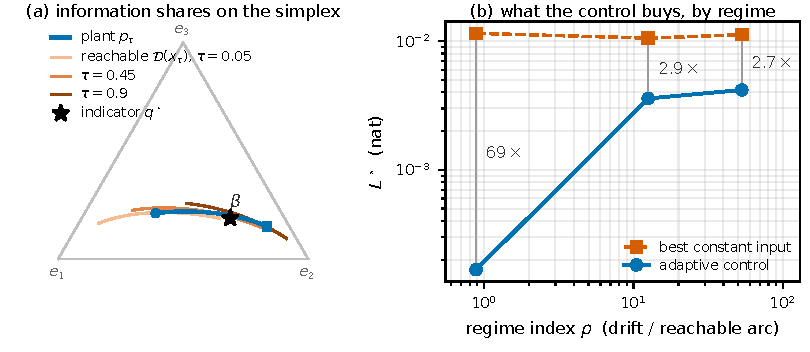
\includegraphics[width=\linewidth]{fig1.pdf}
\caption{(a)~The information-share curve $p_\tau$ on the 2-simplex (circle: start, square: failure), the reachable sets $\mathcal D(x_\tau)$ at $\tau=0.05$, $0.45$ and $0.9$, and the optimal indicator $q^{\star}$. No point lies on all three, so $\beta$ cannot be held at zero (Theorem~\ref{thm:zero}). (b)~What steering buys, against the regime index $\rho$.}
\label{fig:main}
\end{figure}

\subsection{The counting rule, tested in both directions}
\label{sec:counting}

Theorem~\ref{thm:zero} is an equivalence, and the paragraph above tests only
half of it: with too few inputs the floor stays positive. The other half, that
supplying the inputs the counting rule asks for makes the floor vanish, is the
more useful claim for a practitioner deciding how many operating variables to
instrument, so we test it directly.

Give the same three-mechanism plant a second independent input by writing
$\varphi_i(u)=\exp(\theta_i-E_iu_1-G_iu_2)$ with $G=(0.9,0.3,1.2)$, so that
$m=2=d-1$ and each input acts on the mechanisms in a different pattern. Then
$\log\dvec_i$ is affine in $(u_1,u_2)$, and matching a target direction fixes
the $d-1=2$ differences of logarithms: two linear equations in two unknowns,
with a coefficient matrix of determinant $0.27$ here, hence a unique solution
at every state.

Taking as target the direction the plant occupies at mid-life under a central
operating point, that solution lies inside the admissible box $[0,3]^{2}$ at
every one of $600$ sampled states covering the whole life, and the residual
misalignment there is $8.5\times10^{-7}$ degrees, that is, zero to numerical precision; the schedule it requires is drawn in Fig.~\ref{fig:floor}(b). An independent $90\times90$ grid search over the box returns a
floor of at most $0.156^{\circ}$, which is the resolution of the grid rather
than a property of the plant.

The contrast with the single-input case is the content of the theorem: the
same mechanisms, the same shapes, the same envelope on each input, and the
peak floor moves from $4.52^{\circ}$ to zero at every sampled state on the
addition of one operating variable. On this plant the counting rule is
therefore not a conservative sufficient condition but a sharp one, and within the adopted model it fixes how many independent control degrees of freedom the plant must offer. How those degrees of freedom correspond to physical actuators, and how the mechanisms are individuated in the first place, are modelling questions this paper does not settle. Proposition~\ref{prop:contain} says which
plants escape it, and Remark~\ref{rem:family} says why a designer should not
count on being one of them.

\begin{figure}[t]
\centering 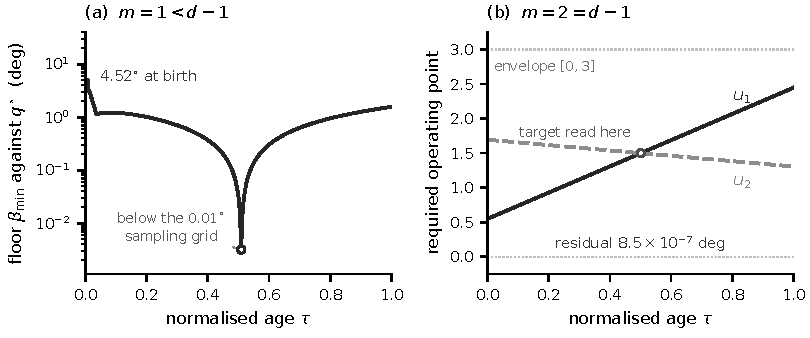
\includegraphics[width=\linewidth]{fig4.pdf}
\caption{(a)~With $m=1$ the floor against $q^{\star}$ is largest at birth and dips below the sampling grid near mid-life. (b)~With $m=2$ the mid-life direction is held exactly; plotted is the operating point this requires, which never leaves $\mathcal U$.}
\label{fig:floor}
\end{figure}

\subsection{The value of steering}
\label{sec:steer}

Minimising over $q$ gives $q^{\star}=(0.466,0.771,0.435)$, at which the
adaptive policy attains $1.68\times10^{-4}$ against $1.15\times10^{-2}$ under the best constant input, a factor of $68$. The ratio depends on how finely
$\mathcal U$ is discretised for the policy, rising to $72$ at $161$ points; we
report it on the $41$-point grid used throughout.

The factor is a ratio of information losses, not of information, and it is not free in reliability terms: the policy that attains it runs the component differently, and Section~\ref{sec:frac} finds the two closed loops separated by a factor of $3.4$ in life. Aligning the indicator and prolonging the component are competing objectives, which is what makes the horizon in \eqref{eq:frac} a controlled quantity rather than a constant. That factor is the value of steering at all, not the value of steering optimally: a myopic policy that attends only to the numerator of
\eqref{eq:frac} sits $2.8\%$ above the optimum at $q^{\star}$.

The fraction in \eqref{eq:frac} is doing visible work at this operating point.
The closed loop at $q^{\star}$ and the closed loop at a balanced indicator,
which calls for far less steering, differ by a factor $3.4$ in lifetime: what
alignment buys in the numerator is paid for in the denominator. This is the
tension anticipated in Section~\ref{sec:limit}, and it is why the horizon
cannot be fixed in advance.

\subsection{The computed fractional optimum}
\label{sec:frac}

Dinkelbach bisection with the control grid matched to the policy gives, over
$N\in\{25,29,35\}$, extrapolants agreeing to $1.2\%$ and
$\lambda^{\star}_\infty=1.63\times10^{-4}$, below the realisable $1.68\times10^{-4}$ as it must be.

We quote this to two digits only, for the following reason: the raw values are
twice the extrapolant, so the first-order correction carries half the answer,
and both quantities still move by $4\%$ between control grids of $41$ and $81$
points. Three checks guard the number: $F$ must decrease and cross zero,
$\lambda^{\star}$ must not exceed a realisable policy, and the grid sequence
must extrapolate consistently. A fixed-horizon formulation failed the second
and third and was discarded, as did a first attempt with mismatched control
grids. A converse bound uniform over trajectories, which would replace this
computation by a theorem, remains open.

\subsection{The regime index, and how far it screens}
\label{sec:regime}

For a practitioner the first question is not how to steer but whether to
bother. One dimensionless ratio answers it. The reachable set $\mathcal D(x)$
is an arc; write $\rho$ for the drift of its midpoint over the life divided by
its mean length, so $\rho$ measures how far the informative direction wanders
in units of the actuation authority available to chase it.

Table~\ref{tab:regime} varies the spread of the activation energies, which by
\eqref{eq:repl} is what sets that authority. As the arc collapses, the
attainable loss $L^{\star}$ rises by a factor $25$ and the value of control
falls from $68$ to $2.7$: with weak authority there is little left to steer.
Fig.~\ref{fig:main}(b) plots the two against $\rho$. The construction of this
paper is a statement about the low-$\rho$ regime, and $\rho$ can be computed
from a nominal degradation model before any indicator is designed.

Three plants differing only in their activation energies are not a screening
law, so the index was tested on $299$ further plants drawn at random: two to
five mechanisms, one or two independently adjustable inputs, and the
pre-exponentials, activation energies, shape coefficients, input envelope,
initial state and signal-to-noise ratio varied together. The rank correlation between $\rho$ and the gain is $-0.36$, with a
bootstrap $95\%$ interval from $-0.46$ to $-0.24$, and it keeps its sign inside
every stratum of the mechanism count and of the input count, so it is not an
artefact of either.

Read as a classifier of whether steering repays a factor of five, which
$32\%$ of the plants do, $\rho$ has an area under the receiver-operating curve
of $0.73$, with interval $0.67$ to $0.79$. The reachable arc alone scores
$0.73$ as well, and the drift alone $0.53$, with interval $0.46$ to $0.60$,
which includes the $0.5$ of a coin toss: most of the index's discriminating
power is in its denominator, and the drift earns its place only among plants
of equal arc. Of the plants below $\rho=2.6$, $52\%$ repay steering fivefold,
against $14\%$ above it, a split read off this same sample and so optimistic. As a veto the index is weaker than that suggests:
rejecting every plant with $\rho\ge1$ would also reject $23\%$ of plants that
would in fact have repaid a factor of five, and that is the expensive error
rather than the cheap one. Nor is lower always better. In the lowest tenth of
$\rho$ only $43\%$ repay fivefold, because there the drift itself is small, a
median of $2.7^{\circ}$ against $14^{\circ}$ over the sample: steering needs
authority, and it also needs something to chase. The first row of
Table~\ref{tab:regime} is not typical of its own regime either: among sampled
plants within a factor $1.4$ of its $\rho$, the median gain is $5.2$ rather
than $68$. $\rho$ describes a regime; it does not decide a design.

\begin{table}[t]
\caption{The regime index. The activation energies $E$ set the actuation authority; $c$, the noise and $\mathcal U$ are held fixed. $L^{\star}$ is the loss under adaptive control, and the gain its ratio to the best constant input.}
\label{tab:regime}
\centering
\begin{tabular}{lcccc}
\hline
$E$ & arc & $\rho$ & $L^{\star}$ & gain\\
\hline
$(0.60,1.10,0.80)$ & $33.9^{\circ}$ & $0.88$ & $1.7\times10^{-4}$ & $68\times$\\
$(0.80,0.82,0.79)$ & $1.93^{\circ}$ & $12.5$ & $3.6\times10^{-3}$ & $2.9\times$\\
$(0.80,0.805,0.798)$ & $0.45^{\circ}$ & $53.1$ & $4.2\times10^{-3}$ & $2.7\times$\\
\hline
\end{tabular}
\end{table}

\subsection{What the loss buys a downstream estimator}
\label{sec:downstream}

Corollary~\ref{cor:mmse} prices the loss in the error of the estimate the model itself prescribes. A practitioner does not use that estimate, so the ordering is worth checking against a procedure that uses none of the construction: sample the indicator over the last $40\%$ of life, match the observed history against the indicator's own reference curve, and read remaining life off the best-fitting time offset. That estimator sees a scalar signal and nothing else --- not $\dhat$, not $\gamma$, not the loss.

Over twelve indicators spanning $\bar\lloss$ from $0.012$ to $0.37$, its median absolute error --- one of the standard prognostic accuracy measures~\cite{saxena2008metrics} --- rises with the loss, at Spearman correlation $0.89$, and the best-aligned indicator beats the worst by a factor $1.5$. Twelve indicators is a small sample, so both are given with intervals obtained by resampling the $160$ units behind each median: $0.34$ to $0.90$ for the correlation, and $1.40$ to $2.03$ for the factor. The ordering is not in doubt --- a one-sided permutation test gives $p=1.5\times10^{-4}$ --- but its strength is, and the point estimate sits near the top of its own interval. The factor is far smaller than the $31$-fold spread in $\bar\lloss$, and it should be: the loss is a logarithmic information quantity, the error is a time, and an estimator with the whole history recovers much of what any one
instant discards.

The same protocol on $120$ further plants, drawn at random as in
Section~\ref{sec:regime}, gives correlations between $0.87$ and $0.99$, with
the plant above among the weaker. That design tilts every indicator toward the
same direction, however, so loss and error both grow with one parameter and
their agreement is close to structural. Tilting instead by a random amount of
up to $60^{\circ}$ in a random direction weakens the median correlation to
$0.74$, with the interval excluding zero on $84\%$ of plants. It also exposes
what the experiment cannot show. On these plants the angle between an
indicator and the mid-life informative direction ranks the indicators
identically to the loss on $82\%$ of plants, with neither consistently better
on the rest, because the direction rotates little beside how far the
indicators differ. The experiment is therefore evidence that the ordering of
the loss carries over to an estimator built from none of this construction; it
is not evidence that the time-averaged loss improves on a mid-life snapshot of
the misalignment, which would need a plant whose direction rotates by more
than its candidate indicators differ.

\section{What public data can say about the premises}
\label{sec:scope}

The construction rests on three modelling choices, and each is empirically
testable. They do not carry equal weight, and Fig.~\ref{fig:scope} separates
what depends on which. Two are premises about the plant: that the informative
direction rotates along the trajectory, and that the input moves it. The third
is the separability of Lemma~\ref{lem:sep}, which is what makes the operator's
authority computable offline. Table~\ref{tab:fleets} summarises what six public run-to-failure
fleets currently settle. Supplementary Section~S1 gives the protocol behind every row, with the parameters of the code that produced it.


\begin{figure*}[tb]
\centering
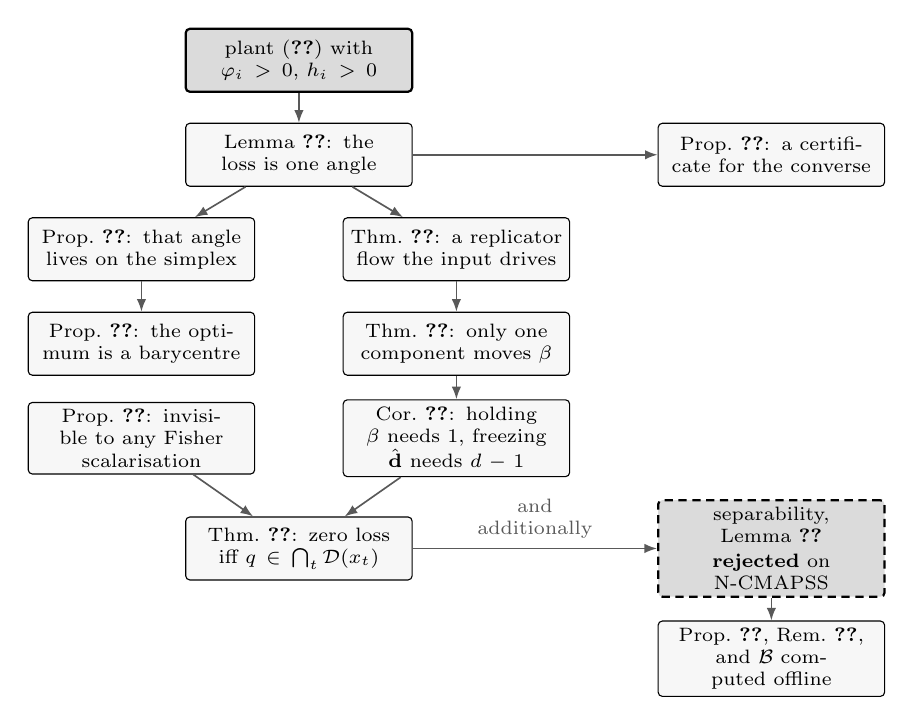
\begin{tikzpicture}[
  font=\small,
  n/.style={draw, rounded corners=1.5pt, align=center, inner sep=2.5pt,
            font=\scriptsize, fill=black!3, minimum height=8mm,
            text width=27mm},
  hyp/.style={n, fill=black!14, thick},
  bad/.style={n, fill=black!14, thick, draw=black, densely dashed},
  e/.style={-{Latex[length=1.6mm]}, semithick, black!65},
  lbl/.style={font=\scriptsize, inner sep=1.5pt}]

% columns at 15 / 55 / 95 mm, so the picture spans 0..110mm
\node[hyp] (mod) at (35mm,0mm)
      {plant \eqref{eq:plant} with $\varphi_i>0$, $h_i>0$};
\node[n] (lem) at (35mm,-12mm)
      {Lemma~\ref{lem:exact}: the loss is one angle};

\node[n] (bha) at (15mm,-24mm)
      {Prop.~\ref{prop:bhat}: that angle lives on the simplex};
\node[n] (bar) at (15mm,-36mm)
      {Prop.~\ref{prop:bary}: the optimum is a barycentre};
\node[n] (bli) at (15mm,-48mm)
      {Prop.~\ref{prop:blind}: invisible to any Fisher scalarisation};

\node[n] (rep) at (55mm,-24mm)
      {Thm.~\ref{thm:repl}: a replicator flow the input drives};
\node[n] (bet) at (55mm,-36mm)
      {Thm.~\ref{thm:beta}: only one component moves $\beta$};
\node[n] (cor) at (55mm,-48mm)
      {Cor.~\ref{cor:tri}: holding $\beta$ needs $1$, freezing $\dhat$ needs
       $d-1$};

\node[n] (con) at (95mm,-12mm)
      {Prop.~\ref{prop:converse}: a certificate for the converse};
\node[n] (zer) at (35mm,-62mm)
      {Thm.~\ref{thm:zero}: zero loss iff $q\in\bigcap_t\mathcal D(x_t)$};

\draw[e] (mod) -- (lem);
\draw[e] (lem) -- (bha);
\draw[e] (lem) -- (rep);
\draw[e] (bha) -- (bar);
\draw[e] (rep) -- (bet);
\draw[e] (bet) -- (cor);
\draw[e] (lem.east) -- (con.west);
\draw[e] (cor) -- (zer);
\draw[e] (bli) -- (zer);

% --------------------------------- the branch that needs more than that ---
\node[bad] (sep) at (95mm,-62mm)
      {separability, Lemma~\ref{lem:sep}\\[1pt]
       \textbf{rejected} on N-CMAPSS};
\node[n] (cnt) at (95mm,-76mm)
      {Prop.~\ref{prop:contain}, Rem.~\ref{rem:family}, and $\mathcal B$
       computed offline};

\draw[e] (zer) -- node[above, font=\scriptsize, align=center] {and\\additionally} (sep);
\draw[e] (sep) -- (cnt);

\end{tikzpicture}
\caption{What rests on what. The spine needs only the positivity of the degradation model. Only the dashed branch adds separability, which Section~\ref{sec:scope} reports as rejected on the best public turbofan data.}
\label{fig:scope}
\end{figure*}

\begin{table*}[tb]
\caption{What the six public fleets settle, and what they cannot. Only the two
turbofan simulations vary the operating point within a unit, which is why the
actuation premise is confirmed in simulation and open on measured hardware.}
\label{tab:fleets}
\centering
\footnotesize
\setlength{\tabcolsep}{3pt}
\begin{tabular}{@{}R{0.16}R{0.14}R{0.31}R{0.34}@{}}
\hline
fleet & premise & what is measured & reading\\
\hline
Severson lithium-ion~\cite{severson2019} & rotation &
arc of an empirically constructed informative direction, the fleet mean, over $\tau\in[0.15,0.9]$, on
$129$ Severson lithium-ion cells &
travels $30.7^{\circ}$ of arc and ends $21^{\circ}$ from its start
(Fig.~\ref{fig:mech}(c)); stays in the open positive orthant once the
window reaches $301$ cycles\\[3pt]
XJTU-SY~\cite{xjtu2020}, PRONOSTIA~\cite{pronostia2012} & actuation &
--- & the operating condition is fixed per unit, so condition and group of
units cannot be separated\\[3pt]
NASA batteries~\cite{saha2007} & actuation & --- & four cells\\[3pt]
C-MAPSS~\cite{saxena2008} & actuation &
between-regime minus within-regime angle, each engine serving as its own
control &
by $7.9^{\circ}$ (FD004) and $10.8^{\circ}$ (FD002), positive for $436$ of $439$ engines; fake regimes give $\lvert B-W\rvert\le0.5^{\circ}$\\[3pt]
N-CMAPSS DS02, DS01~\cite{arias2021} & separability &
interaction against both main effects, in a two-way layout inside engines &
larger by a factor $1.65$ over the operating-point effect on DS02 and $1.84$ on DS01, under every clustering and staging tried: \textbf{rejected}\\
\hline
\end{tabular}
\end{table*}

Three readings qualify the table. The Severson channels are capacity fade,
resistance growth and mean temperature, and mean temperature is a monitoring
channel rather than a damage state --- it is the operating variable itself in
the Arrhenius form of Section~\ref{sec:prelim}. That row therefore reads the
rotation of a direction formed from three measured series, which is what the
premise asserts, and does not need \eqref{eq:obs}'s pairing of channels with
mechanisms. On the four measured fleets the obstacle to testing actuation is
the estimator and not the physics, so the premise is confirmed in simulation
and open on hardware. Both the Severson and the C-MAPSS rows estimate the direction by differentiating each channel along normalised life, which reads a time derivative as the sensitivity of Eq.~\eqref{eq:sens} and so presumes the time-shift population of Section~\ref{sec:prelim}. And the C-MAPSS contrast is reported against a negative control --- fake regimes cut from a single real one, where no contrast exists
by construction --- because a procedure that returned a positive contrast
regardless would produce the same table entry.


The consequence is the scope of the results above. The geometry of
Sections~\ref{sec:simplex} and~\ref{sec:reach} needs only $\varphi_i>0$ and
$h_i>0$, and is untouched. What separability buys, and what the rejection
withdraws, is Proposition~\ref{prop:contain} and the offline route to
$\mathcal B$: those describe a model class, and a plant must be shown to
belong to it before they are used. The two-way layout above is the test, and
it costs one pass over data a reliability programme already holds.

\section{Discussion}
\label{sec:discussion}

Four practical readings follow from the results above. The first two hold
whatever the plant is, because one is a test and the other an invariance. The
last two assume the separable form of \eqref{eq:plant}, which
Section~\ref{sec:scope} reports as rejected on the only data able to test it,
so they apply where that form does and not otherwise.

Test the separability assumption before relying on it. The two-way
layout of Section~\ref{sec:scope} needs only a fleet whose operating point
varies within a unit, and costs one pass over data a reliability programme
already holds. If the interaction clears the measured noise floor, the offline
route to the operator's authority is unavailable and the two model-based
readings below do not apply.

No Fisher criterion can rank fixed indicators by the loss they incur.
This is the second of the two unconditional readings:
Proposition~\ref{prop:blind} is an invariance of the loss under a common gain
and holds whatever the plant, so rules that maximise a scalarisation of the
Fisher information cannot separate configurations whose losses differ by an
order of magnitude. Where the two objectives do coincide, that is a property
of the application, to be verified rather than assumed.

The binding constraint is actuation authority, not indicator
sophistication. Theorem~\ref{thm:zero} prices the operating variables a
lossless fixed indicator would need, and Proposition~\ref{prop:contain}
sharpens the count to sufficient but not necessary, with exceptions that
Remark~\ref{rem:family} shows to be a knife edge. Care in choosing the weights
substitutes for actuation in neither case. What one controllable variable does
buy is the weaker objective of Corollary~\ref{cor:tri}: an installation that
could never freeze the informative direction can still hold the misalignment
constant, though not at zero. Authority bought this way is not free, and
Section~\ref{sec:frac} prices it in life.

The decision to steer precedes the design of the indicator. The regime
index $\rho$ of Section~\ref{sec:regime} requires only a nominal degradation
model and the operating envelope, and Table~\ref{tab:regime} shows the value
of steering collapsing from $68\times$ to under $3\times$ as the reachable arc
shortens relative to the drift. It indicates a regime rather than deciding a design:
Section~\ref{sec:regime} measures how often it is wrong, and in which
direction.

\paragraph{Limitations} Four limitations qualify the readings above. The
separable form of \eqref{eq:plant} is not only an idealisation but one the
data reject: Section~\ref{sec:scope} finds the interaction between operating
point and state larger than either main effect on two N-CMAPSS datasets, so
computing the operator's authority offline is available only where that form
holds. The optimum of Section~\ref{sec:limit} is computed rather than certified, to two digits. The actuation premise is confirmed on simulated rather than measured data, for the reasons set out in Section~\ref{sec:scope}. And the population is taken to slide along one degradation path, which is what makes remaining life a coordinate on it; under dispersion in the coefficients of \eqref{eq:plant} the sensitivity that Remark~\ref{rem:shift} measures stands some $45^{\circ}$ from \eqref{eq:sens}, so the construction describes fleets that vary in when they fail rather than in how they degrade.

\section{Conclusion}
\label{sec:conclusion}

A fixed health indicator discards information, and this paper has treated what
it discards as a quantity the operating point controls. Indicator design then
becomes a reachability question. The family of reachable direction sets bounds what the operating
point can achieve, and their drift relative to their width is a dimensionless
measure, available before any indicator is fixed, of whether substantial
benefit is plausible. Actuation
authority, rather than sophistication of the indicator, governs whether a
fixed compression can come close to lossless. Whether that authority is
present is an empirical question rather than a modelling assumption, and on
$439$ simulated turbofan records it is. Establishing the same on measured
fleets awaits records in which the operating point varies enough to show the
effect.

Section~\ref{sec:scope} rejects that separable form on the
highest-fidelity public turbofan data, so the geometry of
Section~\ref{sec:translate}, and the offline route it opens, describe a model
class rather than measured machinery. What replaces that structure when the
stress model is not separable, and whether a weaker one still yields a
computable reachability criterion, remains open.

Two further questions remain open, the first of them now in a more specific
form. Proposition~\ref{prop:converse} reduces the search for a converse bound
uniform over trajectories to the exhibition of a single continuously
differentiable verification function; the value function is the natural
candidate and fails the differential test for a structural reason, so what is
required is a smooth under-approximation of it, by sum-of-squares programming
or by interval arithmetic with an explicit Lipschitz constant. The other is
unchanged: the computed optimum to better than two digits, which requires a
scheme of higher order than the semi-Lagrangian one used here.

\section*{Data availability and reproducibility}
The six fleets named in Section~\ref{sec:scope} are publicly available. One
script recomputes every reported number from a single configuration and
compares it with the value written in this manuscript and in its
supplementary material, covering the tables and the quantities reported
alongside them; all of its checks pass, and the output of the run that
verified this version is included. The regime-index sweep of
Section~\ref{sec:regime} takes hours, so it and the downstream repeat of
Section~\ref{sec:downstream} are recorded by two further scripts, and the
checks read the records. Three groups of numbers lie outside the checks: the
residuals of the identity checks in Supplementary Section~S4, the barycentre
comparison in Section~\ref{sec:bary}, and the diagnostics of the two candidate
certificates in Supplementary Section~S3. The plots are produced by three
further scripts. All of these are available at
\url{https://github.com/HuyHoangLe0201/health-indicator-information-loss}.

\section*{Declaration of competing interest}
The authors declare that they have no known competing financial interests or personal relationships that could have appeared to influence the work reported in this paper.

\section*{Funding}
This research did not receive any specific grant from funding agencies in the public, commercial, or not-for-profit sectors.

\bibliographystyle{elsarticle-num} \bibliography{Ref}

\end{document}
